\documentclass[11pt,reqno]{amsart}

\usepackage[margin=1.0in]{geometry}
\usepackage{amsmath,amssymb,amsthm,mathtools}
\usepackage{booktabs,array}
\usepackage{graphicx}
\usepackage{xcolor}
\usepackage{hyperref}

\definecolor{navy}{HTML}{0F172A}
\definecolor{accent}{HTML}{1B5E7A}
\hypersetup{
  colorlinks=true,
  linkcolor=accent,
  citecolor=accent,
  urlcolor=accent,
  pdftitle={Tilt Catastrophe, Microscopic Corner Shaving, All-Polygon Rigidity, and the Disk-Limit Paradox for Sobolev Wave Attractors}
}

\newtheorem{theorem}{Theorem}[section]
\newtheorem{proposition}[theorem]{Proposition}
\newtheorem{lemma}[theorem]{Lemma}
\newtheorem{corollary}[theorem]{Corollary}
\theoremstyle{definition}
\newtheorem{definition}[theorem]{Definition}
\theoremstyle{remark}
\newtheorem{remark}[theorem]{Remark}

\newcommand{\R}{\mathbb{R}}
\newcommand{\Z}{\mathbb{Z}}
\newcommand{\N}{\mathbb{N}}
\newcommand{\Q}{\mathbb{Q}}
\DeclareMathOperator{\Fix}{Fix}
\DeclareMathOperator{\dist}{dist}
\DeclareMathOperator{\Id}{Id}

\title[Tilt Catastrophe, Corner Shaving, Rigidity, and Disk-Limit Paradox]{Tilt Catastrophe, Microscopic Corner Shaving,\\
All-Polygon Rigidity, and the Disk-Limit Paradox\\
for Sobolev Wave Attractors}

\author{Project ReMath}
\date{November 24, 2026}
\subjclass[2020]{Primary 35P05, 37E10, 76U05; Secondary 28A78, 37C83, 35L20}
\keywords{Sobolev equation, internal wave attractors, tilted rectangle, Hausdorff dimension, Hecke group, corner shaving, polygon rigidity, regular polygons, quasimodes, Lean~4 formalization}

\setlength{\emergencystretch}{1.2em}
\begin{document}

\begin{abstract}
We investigate how arbitrarily small geometric perturbations---tilting a container, shaving a microscopic corner bevel, or approximating a circular disk by a regular $N$-gon---shatter the standing-wave point spectrum of S.~L.~Sobolev's rotating-fluid operator $T = \Delta_D^{-1}\partial_z^2$ on $H_0^1(\Omega)$ (conjugate via $P\Delta_D = \Delta_D T$ to $P = \partial_z^2\Delta_D^{-1}$ on $H^{-1}(\Omega)$), quantifying the boundary-sensitivity phenomenon first exhibited by R.~A.~Aleksandryan (1949/1960)---who constructed smooth domains arbitrarily close to the disk admitting non-almost-periodic solutions---and developed by T.~I.~Zelenyak (1965/1970). At spectral parameter $E = \lambda^2 \in (0,1)$, the Dirichlet problem $(1-\lambda^2)u_{zz} - \lambda^2 u_{xx} = 0$, $u|_{\partial\Omega} = 0$, reduces to the boundary reflection homeomorphism $b_\lambda = \gamma_\lambda^+\gamma_\lambda^-$ with fixed ray slopes $\pm s$, $s = \tan\theta = \sqrt{1-\lambda^2}/\lambda$, $\lambda = \cos\theta$.

First, for \emph{every fixed} tilted rectangle of aspect ratio $R > 0$ and reduced tilt $0 < \phi < \pi/4$, we prove full-measure wave-attractor capture on the single physical frequency slice: regular periodic attractors occupy exact frequency length $\cos\phi - \sin\phi$ (angular length $\pi/2 - 2\phi$, spectral length $\cos 2\phi$), jumping discontinuously from $0$ at $\phi = 0$ to $1 - O(\phi)$ as $\phi \downarrow 0$, while corner capture fills the complementary measure $1 - \cos\phi + \sin\phi$. Likewise, for \emph{every fixed} horizontal-base right trapezoid, isosceles trapezoid, or sheared parallelogram of wall tilt $\alpha \in (0, \pi/2)$, regular periodic attractors occupy exact frequency length $1 - \sin\alpha$ (angular length $\pi/2 - \alpha$), with corner capture filling $\sin\alpha$. Via Hecke-group coding, holomorphic motion, Harnack's inequality, and strict moving-gap transversality, we prove a uniform Hausdorff-dimension gap $\dim_H E_{R,\phi} \le d_\phi < 1$ (independent of $R$), the exact local dimension identity $\lim_{\varepsilon\downarrow 0}\dim_H(E_{R,\phi} \cap (\theta_c-\varepsilon,\theta_c+\varepsilon)) = \dim_H K_{u(\theta_c)} > 1/2$ at every $\theta_c \in E_{R,\phi}$ (whenever $E_{R,\phi} \ne \varnothing$), and an exact integer tenth-power certificate $\dim_H E_{R,\phi} \le 9/10$ for all $\phi \ge 15^\circ$. We establish the exact five-tank boundary-parity table, finite floor-and-product tongue formulas, the exact spectral extinction law $\sigma_p(T) = \varnothing \iff \cot(2\phi) \le R \le \tan(2\phi)$, geometric re-entry rates near primary tongue edges, small-tilt tongue widths $2\phi/(mn)$, and explicit counterexamples refuting both directions of Zhang--Temnov (2026, Thm.~2.3).

Second, we prove \emph{All-Polygon Rigidity}: among all bounded convex polygons, the axis-aligned rectangle is the unique shape free of both regular hyperbolic attractors and one-sided attracting corners at every transverse slope, via a shallow travel-time obstruction $\dist(n\beta_h, \Z) \le C/n$ (yielding density-$1$ attracting period labels on a square-symmetric chamfered octagon by Hermite--Lindemann). Shaving a single corner of the unit square by equal legs $\varepsilon \downarrow 0$ (area $\varepsilon^2/2 \to 0$) produces exact rational plateaus $[m/n, m/(n-\varepsilon)]$ with $\varepsilon$-independent multiplier $(1-s)/(1+s)$, proving the permanent frequency-measure jump $\liminf_{\varepsilon\downarrow 0} |\mathcal{A}_\varepsilon|_\lambda \ge \frac{6}{\pi^2}(1 - 1/\sqrt{2}) = 0.1780577\ldots$ (and bevel-midpoint factor $\to 1/3$).

Third, we dissect the regular $N$-gon disk limit: exact mod-$4$ corner-capture fractions ($3/N$, $2/N$, $(4/N)(1 - d(0)/h)$), an exact resonance grid and telescoping multiplier law, exact survival of every disk eigenfrequency along $N = 4mq$, a discontinuous zero-tilt Lyapunov cliff ($0 \to -2\log(1+\sqrt{2})$ on polar-angle basin $1/4$) on the regular octagon, a uniform growing-period measure bound $Q = o(N/\sqrt{\log N})$, and the \emph{Half-Frequency Paradox}: at $\lambda = 1/\sqrt{2}$, aligned $N = 4m+2$ polygons have $\ker(T_N - 1/2) = \{0\}$ and $N/2 - 1$ attracting circuits whose strongest factor stays pinned below $1/3$ while $-N\ell_N \Rightarrow 2\pi/\sin(\pi U)$, even as an explicit $H_0^1$ quasimode matches the disk mode $1-r^2$ with residual bound $O(N^{-3/2})$. Core algebraic parity, extinction, microscopic-separation, bevel-multiplier, and mod-$4$ components are formally verified in standalone Lean~4.36.0 with zero \texttt{sorry}.
\end{abstract}

\maketitle

\section{Introduction}

In his 1949 Moscow State University dissertation under S.~L.~Sobolev and his celebrated 1960 monograph-length article \cite{Aleksandryan1960}, R.~A.~Aleksandryan discovered an extraordinary instability of the rotating-fluid spectral problem
\begin{equation}\label{eq:sobolev-p2}
  T u = \lambda^2 u, \qquad T = \Delta_D^{-1}\partial_z^2 \quad \text{on } H_0^1(\Omega),
\end{equation}
which is intertwined with $P = \partial_z^2\Delta_D^{-1}$ on $H^{-1}(\Omega)$ via $P\Delta_D = \Delta_D T$ and corresponds at $E = \lambda^2 \in (0,1)$ to the hyperbolic Dirichlet boundary value problem $(1-\lambda^2)u_{zz} - \lambda^2 u_{xx} = 0$, $u|_{\partial\Omega} = 0$. On the circular disk, Aleksandryan proved that polynomial eigenfunctions form a complete orthogonal basis \cite[\S 9, Thms.~13--14\,bis]{Aleksandryan1960}; yet in his 1949 dissertation (credited in \cite[p.~1225]{Zelenyak1965}) and 1960 paper \cite{Aleksandryan1960}, he constructed smooth domains arbitrarily close to the disk admitting non-almost-periodic solutions, launching the Novosibirsk boundary-sensitivity school of Zelenyak \cite{Zelenyak1965,Zelenyak1970} and Fokin \cite{Fokin1994}. Decades later, oceanographers Maas and Lam \cite{MaasLam1995} and Maas et al.\ \cite{Maas1997} observed that sloping tank walls compress internal-wave beams onto closed periodic \emph{wave attractors}, launching a modern mathematical theory spanning microlocal analysis \cite{CdVSR2020,DyatlovZworski2019,DWZ2025,Li2024} and piecewise-affine circle dynamics \cite{Kopecz2006,BajarsFrankMaas2013,NogueiraTroubetzkoy2020,LBC2023}.

In our companion paper \cite{Paper1}, we established the finite-energy $H_0^1(\Omega)$ polygonal eigenmode criterion, proved the Universal Half-Amplitude Uncloakability Theorem ($\|u\|_{L^\infty(\Gamma)} \ge \frac{1}{2}\|u\|_{L^\infty(\Omega)}$), and solved the fixed-frequency prescribed multi-attractor coexistence problem on convex polygons. Here we examine the \emph{parameter-space and geometric-perturbation anatomy} of polygonal Sobolev tanks, answering three sharp quantitative questions:
\begin{enumerate}
  \item \emph{Fixed-tank tilt catastrophe}: On a \emph{single fixed} tilted rectangle (or horizontal-base trapezoid/shear), what is the exact Lebesgue measure and Hausdorff dimension of frequencies escaping periodic wave attractors? Exactly when does the entire point spectrum $\sigma_p(T)$ go extinct?
  \item \emph{All-polygon rigidity and microscopic corner shaving}: Is the upright rectangle the \emph{unique} convex polygon immune to wave attractors at all frequencies? If one shaves a microscopic triangle of area $\varepsilon^2/2 \to 0$ from a single corner of the unit square, does the attracting frequency measure vanish as $\varepsilon \downarrow 0$ or jump permanently above a positive universal constant?
  \item \emph{Regular $N$-gons approaching the disk}: As $N \to \infty$, how do polygonal attractors, corner trapping, exact surviving eigenfrequencies, and smooth disk quasimodes interact?
\end{enumerate}

\subsection*{Conventions and relation to prior work}
Throughout, $s = \tan\theta = \sqrt{1-\lambda^2}/\lambda > 0$ denotes the physical ray slope ($\lambda = \cos\theta \in (0,1)$, spectral parameter $E = \lambda^2$), characteristics are $\xi = z + sx$, $\eta = z - sx$, and $b_\lambda = \gamma_\lambda^+\gamma_\lambda^-$ first follows a chord of slope $+s$ (preserving $\eta$) and then slope $-s$ (preserving $\xi$). Unless explicitly marked CCW, reduced rational boundary rotation numbers $p/q$ follow the \emph{clockwise} orientation (where $q$ counts two-chord iterations of $b_\lambda$; CCW rotation is $1 - p/q$). We recall from \cite[Thms.~2.1--2.2]{Paper1} that $\ker(T - \lambda^2) \ne \{0\}$ on a convex polygon $K = \overline{\Omega}$ iff $b_\lambda^q|_{\mathcal{C}} = \Id$ on an open boundary arc $\mathcal{C}$ whose full dihedral orbit avoids characteristic edges, in which case $\ker(T - \lambda^2)$ is infinite dimensional.

We carefully distinguish our new theorems from existing results in the literature:
\begin{itemize}
  \item On the tilted square, Kopecz \cite[Thms.~1--3 and p.~9]{Kopecz2006} already derived the primary period-2 tongue, its $\pi/8$ saturation angle, and $k(t_1+t_2) = 1$, while Bajars, Frank, and Maas \cite[\S 2.4]{BajarsFrankMaas2013} discussed the odd--even parity split and the two unbounded winding families $(2k,1)$ and $(1,2k)$.
  \item Nogueira and Troubetzkoy \cite[Thm.~13]{NogueiraTroubetzkoy2020} proved that periodic direction pairs on a square \emph{contain} an open dense subset (allowing two independent ray angles).
  \item Lenci, Bonanno, and Cristadoro \cite[Prop.~3.1, Thm.~3.2, Rem.~3.5, App.~A]{LBC2023} established the wall-section parity theorem, break-return equations, and a \emph{two-parameter} almost-everywhere rational-rotation theorem for rectangular trapezoids via a fixed-dilation surface. For a fixed Hecke group of width $u > 2$, $1/2 < \dim_H \Lambda_u < 1$ is classical \cite{Soares2021}; Zhu (under Z.~Li) \cite[\S 4.1]{ZhuLi2022} gave numerical dimension estimates on tilted squares.
\end{itemize}
Our advances below establish the \emph{single-parameter fixed-tank} full-measure and uniform dimension-gap theorems (including the exact local dimension identity and rational $9/10$ certificate), the unified five-tank boundary-parity table, the exact aspect-ratio extinction law and geometric re-entry asymptotics, global all-polygon rigidity and the $17.80577\%$ microscopic corner-shaving jump, and the exact regular $N$-gon disk-limit laws.

% ==============================================================================
\section{Tilted Rectangles and Canonical Quadrilaterals}\label{sec:tilted}
% ==============================================================================

\subsection{Checkerboard reduction and the five-tank parity table}
Consider a rectangle $[0,1]\times[0,R]$ ($R > 0$) rotated counterclockwise by a reduced tilt $0 < \phi < \pi/4$. (Larger acute tilts map to $(\pi/2 - \phi, 1/R)$ by exchanging body axes; at $\phi = \pi/4$ the open supercritical window is empty and $\theta = \pi/4$ has zero kernel.) For ray angles in the open supercritical window $J = (\phi, \pi/2 - \phi)$, rotating back to body coordinates and rescaling height by $1/R$ yields the unit square with two ray slopes $a$ and $-b_1$, where
\begin{equation}\label{eq:rect-slopes}
  a = \frac{\tan(\theta-\phi)}{R}, \qquad b_1 = \frac{\tan(\theta+\phi)}{R}, \qquad
  \mu = \frac{b_1}{a} = \frac{\sin 2\theta + \sin 2\phi}{\sin 2\theta - \sin 2\phi} > 1.
\end{equation}
Unfolding reflections across all four walls produces a northeast flow on the unit checkerboard with slope $a$ on even cells and $b_1$ on odd cells, invariant under the index-$2$ lattice $L = \{(i,j)\in\Z^2 : i+j\text{ even}\}$. Integrating $1/a$ on the first row and $1/b_1$ on the second, normalized by $1/a + 1/b_1$, converts the column return at $x=0$ modulo $L$ into the two-break circle map $g_{m,t} = T_t \circ J_m$ on $\R/\Z$, where
\begin{equation}\label{eq:two-break}
  m = \frac{b_1}{a + b_1}, \qquad t = \frac{a b_1}{a + b_1}, \qquad
  J_m(y) =
  \begin{cases}
    m + \mu^{-1} y, & 0 \le y \le m, \\
    1 + \mu(y - m), & m \le y \le 1,
  \end{cases}
\end{equation}
extended by degree one ($J_m(y+1) = J_m(y)+1$, $J_m^2 = T_1$).

Similarly, consider the three horizontal-base canonical quadrilaterals of height $H$, mid-height width $W$, and inclined wall departure $\alpha \in (0,\pi/2)$ from vertical ($A = \tan\alpha > 0$, transverse regime $sA < 1$, $\Lambda = (1+sA)/(1-sA) > 1$): the right trapezoid (one inclined wall), isosceles trapezoid (two oppositely inclined walls), and sheared parallelogram (two parallel inclined walls). Writing the affine lateral walls as $L(z) \le x \le R(z)$ and unfolding top and bottom into the $2H$-periodic phase $t$ with physical height $V(t) = \dist(t, 2H\Z)$, the maps $E_X^\pm(t) = t \pm sX(V(t))$ ($X \in \{L, R\}$) are strictly increasing lifts in $sA < 1$, yielding the physical side-to-side lifts $T_{LR} = (E_R^-)^{-1} E_L^-$ and $T_{RL} = (E_L^+)^{-1} E_R^+$ (characterized implicitly by $T_{LR}(t) - t = s[R(V(T_{LR}(t))) - L(V(t))]$ and $T_{RL}(t) - t = s[R(V(t)) - L(V(T_{RL}(t)))]$) and the full left-return lift $F = T_{RL}T_{LR}$, whose section rotation $N/M$ (in units of $2H$) relates to clockwise boundary rotation by $\rho(b) = p/q = N/(M+N)$. Normalizing the period $2H$ to $1$, setting $\tilde a = (1-sA)/2$, $d = 1 - \tilde a = (1+sA)/2$ (so $d/\tilde a = \Lambda$), and defining the degree-one piecewise-affine map
\[
  K_{\tilde a}(t) =
  \begin{cases}
    \tilde a + \Lambda t, & 0 \le t \le \tilde a, \\
    1 + \Lambda^{-1}(t - \tilde a), & \tilde a \le t \le 1,
  \end{cases}
  \qquad (K_{\tilde a}^2 = T_1,\;\; h = T_\delta K_{\tilde a}),
\]
each family conjugates directly to $h = T_\delta K_{\tilde a}$: the right trapezoid has $F \sim h$ ($\delta = sW/H - 1/2$, period $D = M$), the isosceles trapezoid has $F = G^2$ with $G \sim h$ ($\delta = sW/(2H) - 1/2$, $\rho(G) = N/(2M)$), and the sheared parallelogram has $F = G^2 - 1$ with $G \sim h$ ($\delta = sW/(2H)$, $\rho(h) = (M+N)/(2M)$).

\begin{theorem}[Unified five-tank boundary-parity law]\label{thm:five-tanks}
On an upright rectangle ($\phi = 0$), every reduced rational clockwise boundary rotation $p/q$ ($0 < p < q$) occurs at a unique angle $\theta \in (0,\pi/2)$ with $b^q = \Id$ globally and an infinite-dimensional eigenspace, and no attracting or corner-capture frequencies exist. On any of the four non-upright fixed tanks in Table~\ref{tab:five-tanks}, at every rational clockwise boundary rotation $p/q$ ($\gcd(p,q)=1$) attained inside the open supercritical window $J$ ($J = (\phi, \pi/2-\phi)$ for a tilted rectangle, $J = (0, \pi/2-\alpha)$ for a horizontal-base tank):
\begin{enumerate}
  \item Under the parity condition in Column~2 (corresponding to even denominator $D$ of the two-break section $h$), the angle in $J$ is unique, $b^q = \Id$ globally on $\partial\Omega$, and $\ker(T - \lambda^2)$ is infinite dimensional.
  \item Under the complementary parity (odd section denominator $D$), the rational rotation occurs on a nondegenerate tongue that is relatively closed in $J$ (with nonempty open interior in $J$). Throughout its open interior there are unique regular attracting and repelling circuits with the exact full-cycle attracting multiplier in Column~3, every tongue endpoint lying inside $J$ carries a semistable vertex-hitting cycle, and $\ker(T - \lambda^2) = \{0\}$ on the entire tongue.
  \item Every irrational rotation frequency, every critical edge-parallel angle (for instance $\theta = \phi$ on a tilted square with $R = 1$, $\tan(2\phi) = 2$, where the midpoint-extended boundary map carries the primitive vertex cycle $(0,0) \mapsto (1/2,1) \mapsto (1,0) \mapsto (0,0)$), and every angle in the open corner-capture bands satisfies $\ker(T - \lambda^2) = \{0\}$.
\end{enumerate}
\end{theorem}

\begin{table}[ht]
\centering
\caption{Unified boundary-parity classification for all five canonical quadrilateral families (clockwise reduced boundary rotation $p/q$, $\Lambda = (1+s\tan\alpha)/(1-s\tan\alpha)$, $\mu = \tan(\theta+\phi)/\tan(\theta-\phi)$). At $H = W$, $\lambda = 1/\sqrt{2}$ ($s=1$), $\alpha = \phi = 15^\circ$, the five full-cycle multipliers equal $1,\; 1/\sqrt{3},\; 1,\; 1/3,\; 1/9$ (Figure~\ref{fig:p2-fig1}B inset).}
\label{tab:five-tanks}
\footnotesize
\setlength{\tabcolsep}{4pt}
\begin{tabular}{@{}llll@{}}
\toprule
Tank geometry & Globally neutral ($b^q=\Id$) & Regular attracting multiplier & Corner-capture angles \\
\midrule
Upright rectangle ($\phi=0$) & Every rational $p/q$ & None (all multipliers $1$) & None \\
Right trapezoid (1 wall $\alpha$) & $q - p$ even & $\Lambda^{-1}$ ($q-p$ odd, tongue int.) & $\theta > \pi/2 - \alpha$ \\
Isosceles trapezoid ($/\ \backslash\ \alpha$) & $p$ odd & $\Lambda^{-2}$ ($p$ even, tongue int.) & $\theta > \pi/2 - \alpha$ \\
Sheared parallelogram ($/\ /\ \alpha$) & $q$ odd & $\Lambda^{-2}$ ($q$ even, tongue int.) & $\theta > \pi/2 - \alpha$ \\
Tilted rectangle ($0<\phi<\pi/4$) & $q$ odd & $\mu^{-2}$ ($q$ even, tongue int.) & $\theta < \phi$ or $\theta > \pi/2 - \phi$ \\
\bottomrule
\end{tabular}
\end{table}

\begin{proof}
For the upright rectangle ($\phi = 0$), the boundary metric $d\ell_s = s|dx| + |dz|$ makes both chord involutions isometric and $b_\lambda$ a rigid translation of clockwise rotation $sW/(H+sW)$, giving the first statement immediately. For the four non-upright tanks, in the normalized two-break map $h = T_\delta K_{\tilde a}$ of period $D$, a $D$-periodic orbit cuts the circle into $D$ transitively permuted gaps. Because $h$ has only two breaks with opposite log-slope jumps $\pm 2\log\Lambda$ (or $\pm 2\log\mu$), the log-derivative of $h^D$ on each gap takes two neighboring integer multiples of $\log\Lambda$ of the same parity as $D$, while the mean slope across each gap equals $1$. For even $D$, the slope is identically $1$, forcing $h^D = \Id$ globally; for odd $D$, the two slopes in each gap are $\Lambda^{-1}$ and $\Lambda$, yielding one regular attracting cycle (multiplier $\Lambda^{-1}$) and one repelling cycle ($\Lambda$) when neither break is periodic, and a semistable vertex cycle at each tongue endpoint inside $J$ \cite[Prop.~3.1]{LBC2023}. Converting section period $D$ to clockwise boundary rotation $p/q = N/(M+N)$: for the right trapezoid $D = M = q - p$ (one physical lap, factor $\Lambda^{-1}$); for the isosceles trapezoid $\rho(G) = N/(2M)$, so $D$ is odd iff $p = N$ is even, and the physical return $F = G^2$ traverses two model laps (factor $\Lambda^{-2}$); for the shear and tilted rectangle, $\rho(h) = (M+N)/(2M)$, so $D$ is odd iff $q = M+N$ is even, again traversing two model laps (factors $\Lambda^{-2}$ and $\mu^{-2}$).

To verify uniqueness of every neutral angle and nondegeneracy of every odd-$D$ tongue, we establish strict parameter monotonicity in the \emph{physical} return coordinates before applying any parameter-dependent conjugacy (note that the conjugated map $g_{m,t}(0)$ need not be monotone in $\theta$). On a tilted rectangle, the unfolded checkerboard column exit $Y$ from entry height $y$ satisfies $\int_y^Y S_\theta(u)^{-1}\,du = 1$, where the local cell slope $S_\theta \in \{a(\theta), b_1(\theta)\}$ increases strictly in $\theta$ on both cell colors; hence $Y$ increases strictly in $\theta$. On each horizontal-base tank, $T_{LR}(t) - t = s[R(V(T_{LR}(t))) - L(V(t))] > 0$ while $t \mapsto t - sR(V(t))$ is strictly increasing, so raising $s$ strictly raises $T_{LR}(t)$ and similarly $T_{RL}(t)$, making the physical lift $F = T_{RL}T_{LR}$ strictly increasing in $s$. Comparing complete iterates rules out two distinct angles carrying $b^q = \Id$, and guarantees that every attained odd-$D$ rotation spans a nondegenerate tongue relatively closed in $J$ whose interior endpoints in $J$ are break-periodic (semistable) cycles. Zero kernel at critical angles ($sA = 1$, or $\theta \in \{\phi, \pi/2-\phi\}$) follows by propagating boundary constancy of $A(\xi) = B(\eta)$ across the characteristic side and the two parallel horizontal (or opposite) walls; zero kernel on corner bands and irrational rotations follows from \cite[Thms.~2.2--2.3]{Paper1}.
\end{proof}

Note the striking geometric reversal at $H = W$, $\lambda = 1/\sqrt{2}$, $\alpha = \phi = 15^\circ$ (clockwise rotation $1/2$, Figure~\ref{fig:p2-fig1}B inset): tilting one wall gives contraction $1/\sqrt{3}$; tilting the opposite wall symmetrically into an isosceles trapezoid \emph{restores} global neutrality $b^2 = \Id$ (factor $1$); tilting it parallel into a shear squares the contraction to $1/3$; and rotating the entire square by $15^\circ$ squares it again to $1/9$!

\subsection{Exact finite tongue equations and complete rotation range}
For the tilted rectangle with coprime unfolded winding $(m,n)$ ($q = m+n$, $P/D = (m+n)/(2m)$ in lowest terms), the exact tongue boundaries admit a closed finite arithmetic expression.

\begin{theorem}[Finite floor-and-product tongue formula and rotation range]\label{thm:tongue-formula}
For any stretch parameter $\sigma > 0$, set $l_\sigma = \sigma/(1+\sigma)$, and for $0 \le j \le D-1$ define $r_j = jP \bmod D$, $d_j = \lfloor (j+1)P/D \rfloor - \lfloor jP/D \rfloor$,
\[
  (s_j, c_j) =
  \begin{cases}
    (\sigma^{-1},\, l_\sigma), & 2r_j < D, \\
    (\sigma,\, 1 - \sigma l_\sigma), & 2r_j \ge D,
  \end{cases}
  \qquad W_j = \prod_{k=j+1}^{D-1} s_k, \qquad
  C_\sigma(P,D) = \frac{\sum_{j=0}^{D-1} W_j (d_j - c_j)}{\sum_{j=0}^{D-1} W_j}.
\]
Then the tilted rectangle realizes CCW boundary rotation $m/(m+n)$ (CW rotation $n/(m+n)$) in $J = (\phi, \pi/2-\phi)$ if and only if $t = ab_1/(a+b_1)$ lies in the closed interval between $C_\mu(P,D)$ and $C_{\mu^{-1}}(P,D)$ (distinct for odd $D$, coinciding for even $D$). In particular, across $J$, the complete set of attained clockwise boundary rotation numbers is precisely
\begin{equation}\label{eq:rot-range}
  \rho_{\mathrm{CW}}(b_\lambda) \in \left[ \frac{1}{2\lceil R\cot(2\phi) \rceil},\;\; 1 - \frac{1}{2\lceil \cot(2\phi)/R \rceil} \right].
\end{equation}
\end{theorem}

\begin{proof}
At a tongue boundary, one of the two breaks ($0$ or $m$) of $g_{m,t} = T_t J_m$ is $D$-periodic. Starting at the break $0$, the cyclic ranks of its iterates are $r_j = jP \bmod D$ with integer carries $d_j$. For odd $D$, the right return slope at $0$ is $\sigma^{-1}$ and the left slope is $\sigma$, forcing exactly the first $(D+1)/2$ ranks ($2r_j < D$) onto the first branch; for even $D$, exactly $D/2$ ranks lie there (using right derivatives). Solving the affine recurrence $x_{j+1} = s_j x_j + c_j + t - d_j$ with $x_0 = x_D = 0$ yields $t = C_\mu(P,D)$; translating the second break $m$ to $0$ replaces $\mu$ by $\mu^{-1}$. For the boundary families $n = 1$, $m = 2k+1$, this reduces to $(k+1)a + k b_1 \le 1 \le k a + (k+1)b_1$, while for $m = 2k$ it gives $k(a+b_1) = 1$. As $\theta \downarrow \phi$, $(a, b_1) \to (0, \tan(2\phi)/R)$, placing $\theta = \phi+$ in the band $k = \lceil R\cot(2\phi) \rceil - 1$ (clockwise rotation $1/(2k+2)$); exchanging axes ($R \mapsto 1/R$) gives the upper endpoint in \eqref{eq:rot-range}.
\end{proof}

\subsection{Fixed-slice full-measure capture and uniform Hausdorff dimension gap}
A two-parameter almost-everywhere theorem \cite[Thm.~3.2]{LBC2023} leaves open whether a \emph{specific} physical tank (such as the $15^\circ$-tilted unit square) could lie in a measure-zero exceptional slice. We rule this out for \emph{every} fixed tank and determine the sharp fractal dimension of the exceptional set.

\begin{theorem}[Fixed-slice full measure, uniform dimension gap, and local dimension identity]\label{thm:measure-dim}
Fix any aspect ratio $R > 0$ and reduced tilt $0 < \phi < \pi/4$. Let $E_{R,\phi} \subset J = (\phi, \pi/2 - \phi)$ be the set of supercritical angles lacking a regular hyperbolic periodic attractor.
\begin{enumerate}
  \item \textbf{Full-measure jump on every fixed slice}: The regular periodic-attractor set $J \setminus E_{R,\phi}$ has exact Lebesgue measure $\pi/2 - 2\phi$ in $\theta$, $\cos\phi - \sin\phi$ in physical frequency $\lambda$, and $\cos(2\phi)$ in spectral parameter $E = \lambda^2$. Corner capture fills the complementary measures $2\phi$, $1 - \cos\phi + \sin\phi$, and $1 - \cos(2\phi)$. Thus the periodic-attractor frequency measure jumps discontinuously from $0$ at $\phi = 0$ to $\cos\phi - \sin\phi \to 1$ as $\phi \downarrow 0$, uniformly in $R$. Likewise, every fixed horizontal-base right trapezoid, isosceles trapezoid, or shear with wall tilt $\alpha \in (0,\pi/2)$ has regular-attractor measure $1 - \sin\alpha$ in $\lambda$ (and $\pi/2 - \alpha$ in $\theta$).
  \item \textbf{Uniform Hausdorff dimension gap and exact local dimension}: There exists $d_\phi < 1$, depending only on $\phi$ (independent of $R$), such that
  \begin{equation}\label{eq:dim-gap}
    \dim_H E_{R,\phi} \le d_\phi < 1.
  \end{equation}
  Whenever $E_{R,\phi} \ne \varnothing$, every point $\theta_c \in E_{R,\phi}$ obeys the exact local dimension identity
  \begin{equation}\label{eq:local-dim}
    \lim_{\varepsilon \downarrow 0} \dim_H\bigl(E_{R,\phi} \cap (\theta_c - \varepsilon, \theta_c + \varepsilon)\bigr) = \dim_H K_{u(\theta_c)} > \frac{1}{2},
  \end{equation}
  where $K_u$ is the Hecke continued-fraction limit set at width $u(\theta) = \sqrt{\mu} + \sqrt{\mu^{-1}} \ge 2\sec(2\phi) > 2$.
  \item \textbf{Explicit rational certificate}: For every $\phi \in [15^\circ, 45^\circ)$ and every $R > 0$, $\dim_H E_{R,\phi} \le 9/10$.
\end{enumerate}
\end{theorem}

\begin{proof}
(\emph{Step 1: Hecke-group coding}) Set $r = \sqrt{a/b_1} \in (0,1)$, $x = \sqrt{ab_1}$, and
\[
  u = r + r^{-1} = \frac{2\sin(2\theta)}{\sqrt{\sin^2(2\theta) - \sin^2(2\phi)}} \ge u_* := 2\sec(2\phi) > 2, \qquad t = \frac{x}{u}.
\]
At fixed $u > 2$, three operations preserve regular hyperbolic pairs and finite order of $g_{m,x/u}$: (i) translation $x \mapsto x + u$, (ii) sign flip $x \mapsto -x$ (conjugating $g_{m,x/u}$ to its inverse), and (iii) checkerboard transposition $x \mapsto 1/x$ ($x > 0$, exchanging colors and horizontal/vertical sections). The primary tongue $a < 1 < b_1$ is precisely $r < x < r^{-1}$. Applying nearest-multiple reduction $y_0 = x - n_0 u \in [-u/2, u/2]$ and iterating $y_{j-1} = \psi_{n_j, u}(y_j) := -1/(n_j u + y_j)$ ($n_j \in \Z \setminus \{0\}$) whenever $0 < |y_{j-1}| \le r$ shows that $x$ escapes all regular hyperbolic orbits iff $x \in u\Z + K_u$, where $K_u$ is the union of $0$, all finite compositions $\psi_{w,u}(0)$, and all infinite limits $\lim_{k\to\infty}\psi_{w|_k, u}(0)$ (since finite codes reduce to $g_{m,0} = J_m$ of order $2$, and regular hyperbolicity is open in $x$ while finite truncations approximate every infinite code). Thus $E_{R,\phi} = \{\theta \in J : x(\theta) \in u(\theta)\Z + K_{u(\theta)}\}$.

(\emph{Step 2: Uniform fiber dimension $d_\phi < 1$ and lower bound $> 1/2$}) On $I = [-1,1]$, for all $u \ge u_* > 2$, the first-level images $\psi_{n,u}(I)$ are disjoint inside $[-t_0, t_0]$ ($t_0 = 1/(u_*-1) < 1$) with uniform contraction $L = t_0^2 < 1$ and distortion bound $D = \exp(4t_0/(1-L))$ (from $|\partial_z \log \psi'_{n,u}(z)| \le 2t_0$). Each cylinder loses at least fraction $\eta = (1-t_0)/D > 0$ of its length, giving $\sum_{|w|=k} \sup_I \psi'_{w,u} \le D(1-\eta)^k < 1$ for a fixed block length $k$ depending only on $u_*$. Dominated convergence using the uniform tail bound $\sum_{n\ne 0}(|n|u_*-1)^{-2d_0} < \infty$ ($d_0 > 1/2$) yields $d_\phi < 1$ with $\sup_{u \ge u_*} \sum_{|w|=k} (\sup_I \psi'_{w,u})^{d_\phi} < 1$, hence $\dim_H K_u \le d_\phi$ uniformly in $u \ge u_*$. Conversely, for each fixed $u > 2$, $\sum_{n\ne 0} (|n|u+1)^{-1} = \infty$, so a finite alphabet $S$ and $s > 1/2$ satisfy $\sum_{n\in S} (|n|u+1)^{-2s} > 1$; assigning independent weights proportional to $(|n|u+1)^{-2s}$ gives $\dim_H K_u \ge s > 1/2$ by the mass distribution principle.

(\emph{Step 3: Holomorphic motion, Harnack inequality, and strict moving-gap transversality}) On the half-plane $\operatorname{Re} u > 2$, each code value $h_w(u)$ is holomorphic and distinct codes remain strictly separated (since $|(n-n')u| > 2$ and no nonempty tail vanishes). Fix $\theta_c \in J$ and a small complex disk around $\theta_c$ where $x, u$ are holomorphic and $\operatorname{Re} u > 2$. For any two distinct codes $w, v$ with base coordinates $z = h_w(u(\theta_c))$ and $z' = h_v(u(\theta_c))$, applying Harnack's inequality to the positive harmonic function $\log(3/|h_w(u(\zeta)) - h_v(u(\zeta))|)$ on a concentric disk of relative radius $\rho < 1$ gives the two-sided uniform H\"older bounds
\[
  |h_w(u(\zeta)) - h_v(u(\zeta))| \le 3^{1-\alpha}|z - z'|^\alpha, \qquad
  |z - z'| \le 3^{1-\alpha}|h_w(u(\zeta)) - h_v(u(\zeta))|^\alpha, \qquad \alpha = \frac{1-\rho}{1+\rho},
\]
with $\alpha \uparrow 1$ as $\rho \downarrow 0$ (and Cauchy's integral formula on a slightly smaller concentric disk yields a forward H\"older bound with exponent $\alpha$ for the code derivatives $\partial_\theta h_w(u(\theta))$).

Crucially, along any connected positive piece of a code curve $H(u) = n_0 u + h_w(u)$, the associated speeds $A = r H$ and $B = H/r$ cannot both increase strictly: for a finite code the section has constant rational rotation, whereas strictly increasing both speeds strictly raises every output of the travel-time lift and cannot preserve a finite-order rotation number; infinite codes inherit this monotonicity obstruction by uniform convergence of finite truncations. Meanwhile along the physical curve both $a'(\theta) > 0$ and $b_1'(\theta) > 0$. Setting $F(\theta, z) = x(\theta) - H(u(\theta))$ and differentiating $a - A = r F$, $b_1 - B = F/r$ at any crossing $F = 0$ yields the strict uniform transversality
\[
  \partial_\theta F \ge \min(a'/r,\, r b_1') > 0.
\]
Thus each code crosses the physical curve at most once, and near any incidence $\theta_c \in E_{R,\phi}$ the implicit crossing map $z \mapsto \theta(z)$ is bi-H\"older with exponent $\alpha$ arbitrarily close to $1$. Since every relative neighborhood in $K_u$ contains a bi-Lipschitz M\"obius image of all of $K_u$, letting $\alpha \uparrow 1$ proves both \eqref{eq:local-dim} and \eqref{eq:dim-gap} (hence $|E_{R,\phi}| = 0$). For every fixed horizontal-base tank, taking the positive translation lift $\delta = C + D s > 0$ (namely $\delta = \frac{1}{2} + sW/H$ for the right trapezoid, $\frac{1}{2} + sW/(2H)$ for the isosceles trapezoid, and the unshifted $\delta = sW/(2H)$ with $C = 0$ for the shear) gives checkerboard speeds $U_* = \delta/(1-\tilde a)$ and $V_* = \delta/\tilde a$ whose derivatives have the signs of $D - AC$ and $D + AC$; both are strictly positive (from positive shorter base $W/H > A/2$ for the right trapezoid and $W/(2H) > A/2$ for the isosceles trapezoid, and directly from $D = W/(2H) > 0$, $C = 0$ for the shear), so the identical moving-gap transversality gives full regular-attractor measure $1 - \sin\alpha$ in $\lambda$.

(\emph{Step 4: Exact $9/10$ integer certificate}) For $\phi \ge 15^\circ$, we have $u \ge L = 4/\sqrt{3}$. Restrict the domain of the branches $\psi_{n,u}$ to the invariant subinterval $I_0 = [-d_0, d_0]$ with $d_0 = 1/\sqrt{3}$; indeed, for every $u \ge L$, $n \in \Z \setminus \{0\}$, and $z \in I_0$,
\[
  |\psi_{n,u}(z)| = \frac{1}{|nu + z|} \le \frac{1}{L - d_0} = \frac{1}{4/\sqrt{3} - 1/\sqrt{3}} = \frac{1}{\sqrt{3}} = d_0,
\]
so $\psi_{n,u}(I_0) \subseteq I_0$. On $I_0$, every single-digit derivative satisfies $\sup_{I_0} \psi'_{n,u} \le (|n|L - d_0)^{-2} = 3/(4|n|-1)^2 =: M_n$, and multiplying three fractional-linear matrices bounds the derivative supremum of every 3-digit word $(i,j,k) \in (\Z\setminus\{0\})^3$ uniformly on $I_0$ and $u \in [L,\infty)$ by
\[
  M_{ijk} = \frac{27}{\bigl(|64ijk - 12i - 12k| - |16ij - 3|\bigr)^2}.
\]
Setting $t = 9/10$ and $N = 24$, summing all $(2N)^3 = 110{,}592$ finite triples and bounding the tail by $3S^2 T + 3ST^2 + T^3$ (where $S = 2\sum_{n=1}^N M_n^t$ and $T = (4N-1)M_N^t/[2(2t-1)]$) via exact integer tenth-power upward rounding at resolution $10^{-12}$ certifies $\sum_{i,j,k} M_{ijk}^{9/10} \le 0.990179874 < 991/1000 < 1$ (\texttt{experiments/phase1\_canonical.py}), proving $\dim_H E_{R,\phi} \le 9/10$ for all $\phi \ge 15^\circ$ and $R > 0$.
\end{proof}

\subsection{Exact spectral extinction, geometric re-entry, small-tilt asymptotics, and refutation of Zhang--Temnov (2026)}

\begin{theorem}[Spectral extinction, re-entry law, and small-tilt tongue scaling]\label{thm:extinction-reentry}
Let $\Omega_{R,\phi}$ be a rectangle of aspect ratio $R > 0$ at reduced tilt $0 < \phi < \pi/4$.
\begin{enumerate}
  \item \textbf{Exact spectral extinction}: The point spectrum satisfies
  \begin{equation}\label{eq:extinction}
    \sigma_p(T) = \varnothing \quad \Longleftrightarrow \quad \cot(2\phi) \le R \le \tan(2\phi).
  \end{equation}
  Outside this closed horn (Figure~\ref{fig:p2-fig1}B), $\sigma_p(T)$ is countably infinite and every eigenvalue has infinite multiplicity. For a square ($R = 1$), the last standing eigenvalue dies sharply at $\phi = 22.5^\circ$.
  \item \textbf{Geometric re-entry rate}: Whenever $R > \tan(2\phi)$, the lower primary-tongue endpoint $\theta_0 = \arctan R - \phi \in J$ is approached from below by an explicit sequence of globally neutral standing angles $\theta_N$ of period $2N+1$ solving $b_1(\theta_N) = (1 - r^{2N})/(1 - r^{2N+2})$, obeying the exact geometric convergence law ($t_0 = \tan 2\phi$):
  \begin{equation}\label{eq:reentry}
    \theta_0 - \theta_N \sim \frac{t_0}{1 + R t_0} \left( \frac{R - t_0}{R(1 + R t_0)} \right)^N \qquad (N \to \infty).
  \end{equation}
  (By $R \mapsto 1/R$, a symmetric sequence approaches $\theta_1 = \arctan R + \phi$ from above when $R < \cot(2\phi)$.)
  \item \textbf{Small-tilt paradox}: For fixed coprime odd $(m,n)$, the individual tongue around $\theta_* = \arctan(Rn/m)$ shrinks linearly as $\theta_\pm = \theta_* \pm \phi/(mn) + O_{R,m,n}(\phi^2)$. Letting $A_Q(\phi, R)$ denote the total angular measure of hyperbolic tongues with boundary period $q = m + n \le Q$, for every fixed $Q$ we have $\lim_{\phi\downarrow 0} A_Q(\phi,R)/\phi = 2\sum_{m+n\le Q,\,(m,n)=1,\,m,n\text{ odd}} (mn)^{-1} \sim \frac{4}{\pi^2}(\log Q)^2$ (as $Q \to \infty$), and the entire primary family $E_1 = \{m=1 \text{ or } n=1\}$ occupies only $|E_1|_\theta = 2\phi\log(1/\phi) + O_R(\phi)$---even though the full union across all periods jumps immediately to measure $\pi/2 - 2\phi$!
\end{enumerate}
\end{theorem}

\begin{proof}
By \eqref{eq:rot-range}, the supercritical rotation interval reduces to the single value $\{1/2\}$ iff $\lceil R\cot(2\phi) \rceil = \lceil \cot(2\phi)/R \rceil = 1$, i.e., $\cot(2\phi) \le R \le \tan(2\phi)$. In that case the primary tongue fills $J$, leaving no odd-denominator rational rotations and hence $\sigma_p(T) = \varnothing$ by Theorem~\ref{thm:five-tanks}. Otherwise the rotation range is a nondegenerate interval containing countably infinitely many odd-denominator rationals, each yielding an infinite-dimensional eigenspace. For~(2), the finite Hecke iterates $h_N(u) = \psi_{-1,u}^N(0) = r(1-r^{2N})/(1-r^{2N+2})$ satisfy $x = h_N(u) \iff b_1 = (1-r^{2N})/(1-r^{2N+2})$ with primitive winding $(2N+2, 2N)$ and boundary period $2N+1$. Expanding $1 - b_1(\theta_N) = r_N^{2N}(1-r_N^2)/(1-r_N^{2N+2})$ around $b_1(\theta_0) = 1$ using $b_1'(\theta_0) = (1+R^2)/R$ and $r(\theta_0)^2 = (R - t_0)/(R(1 + R t_0))$ yields \eqref{eq:reentry} (verified at $5^\circ$ square, $N = 64$, with ratio $0.999999999958$; Figure~\ref{fig:p2-fig2}C).

For~(3), set $u_0 = \tan\theta/R$ at fixed coprime odd $(m,n)$; then $t = u_0/2 + O(\phi^2)$ and the break location $l = b_1/(a+b_1)$ equals $1/2 + \epsilon$ with $\epsilon = \phi\sec^2\theta/(2\tan\theta) + O(\phi^2)$. Uniformly on $\R/\Z$, $J_l(x) = x + 1/2 + \epsilon\tau(x) + O(\epsilon^2)$, where $\tau$ is the $1$-periodic continuous triangular wave given by $\tau(x) = 1 - 4x$ on $[0,1/2]$ and $\tau(x) = 4x - 3$ on $[1/2,1]$. For odd $m$ and $\gcd(P,m)=1$, summing $\sum_{j=0}^{m-1}\tau(x + jP/m) = \tau(mx)/m$ gives break shifts $\pm\epsilon/m^2 + O(\epsilon^2)$ in $t$; dividing by $dt/d\theta = \sec^2\theta/(2R)$ at $\phi = 0$ yields $\theta_\pm = \theta_* \pm \phi/(mn) + O_{R,m,n}(\phi^2)$. Summing these widths over all coprime odd pairs with $m + n \le Q$ gives the stated limit of $A_Q(\phi, R)/\phi$; bracketing the triangle $m + n \le Q$ between $[1, Q/2]^2$ and $[1, Q]^2$ and applying M\"obius inversion over odd common divisors yields the successive-limit coefficient $2 \cdot \frac{1}{4}\prod_{p\text{ odd}}(1 - p^{-2}) = 4/\pi^2$. To evaluate $|E_1|_\theta$ uniformly as $\phi \downarrow 0$ (without summing the fixed-$(m,n)$ remainder), rewrite the shallow primary-family condition $(k+1)a + kb_1 \le 1 \le ka + (k+1)b_1$ ($m = 2k+1 \ge 3, n = 1$) as $|m\sin 2\theta - R\cos 2\theta - R\cos 2\phi| \le \sin 2\phi$, whose unclipped endpoints are
\[
  \theta_\pm = \frac{1}{2}\left(\arctan\frac{R}{m} + \arcsin\frac{R\cos 2\phi \pm \sin 2\phi}{\sqrt{m^2 + R^2}}\right).
\]
Intersecting with $J$, all $1 \le k < R\cot(2\phi)$ contribute (with at most the terminal tongue clipped), and the mean-value theorem gives the uniform unclipped width $\theta_+ - \theta_- = \frac{\sin 2\phi}{m}[1 + O_R(m^{-2})]$. Summing $1/m$ over odd $m \le O_R(1/\phi)$ yields $\frac{1}{2}\log(1/\phi) + O_R(1)$, giving $\phi\log(1/\phi) + O_R(\phi)$ for the shallow family; reflecting via $R \mapsto 1/R$ doubles this (counting the central $m=n=1$ tongue once), proving $|E_1|_\theta = 2\phi\log(1/\phi) + O_R(\phi)$.
\end{proof}

\begin{remark}[Exact refutation of Zhang--Temnov (2026, Theorem~2.3)]\label{rem:zt}
Theorem~2.3 of Zhang and Temnov \cite{ZhangTemnov2026} proposes commensurability of a local body-coordinate ray slope with $H/L$ as an eigenvalue criterion for the constant-coefficient Dirichlet streamfunction problem in a tilted rectangle (their squared frequency is $\sin^2\theta = 1 - E$, agreeing with ours at $E = 1/2$). Both implications fail because reflection exchanges two \emph{different} body-coordinate slopes $a \ne b_1$:
\begin{itemize}
  \item \emph{Rational slopes, no eigenvalue}: On the unit square tilted by $\tan\phi = 1/3$ at $\lambda^2 = 1/2$ ($\theta = \pi/4$), the two local ray slopes are exact rationals $1/2$ and $-2$, yet exhaustive rational subdivision of the boundary into 12 affine intervals (and Lean~4 theorem \texttt{square\_period\_two\_iff} in \texttt{TiltedParity.lean}) proves that $b^2$ has exactly four fixed points at perimeter coordinates $1/3, 7/3$ (multiplier $1/16$) and $4/3, 10/3$ (multiplier $16$), measured counterclockwise from the bottom-left vertex, with no fixed interval and hence $\ker(T - 1/2) = \{0\}$. Likewise $\tan\phi = 1/2$, $\theta = \pi/4$ has rational local slopes $1/3, -3$ and attracting multiplier $1/81$.
  \item \emph{Irrational slopes, infinite-dimensional eigenspace}: Taking $a = \sqrt{2} - 1$ and $b_1 = 2 - \sqrt{2}$ (both irrational!) satisfies $a + b_1 = 1$, which by Theorem~\ref{thm:tongue-formula} gives $b^3 = \Id$ globally and an infinite-dimensional space of $C^\infty$ eigenmodes.
\end{itemize}
\end{remark}

\begin{figure}[ht]
\centering
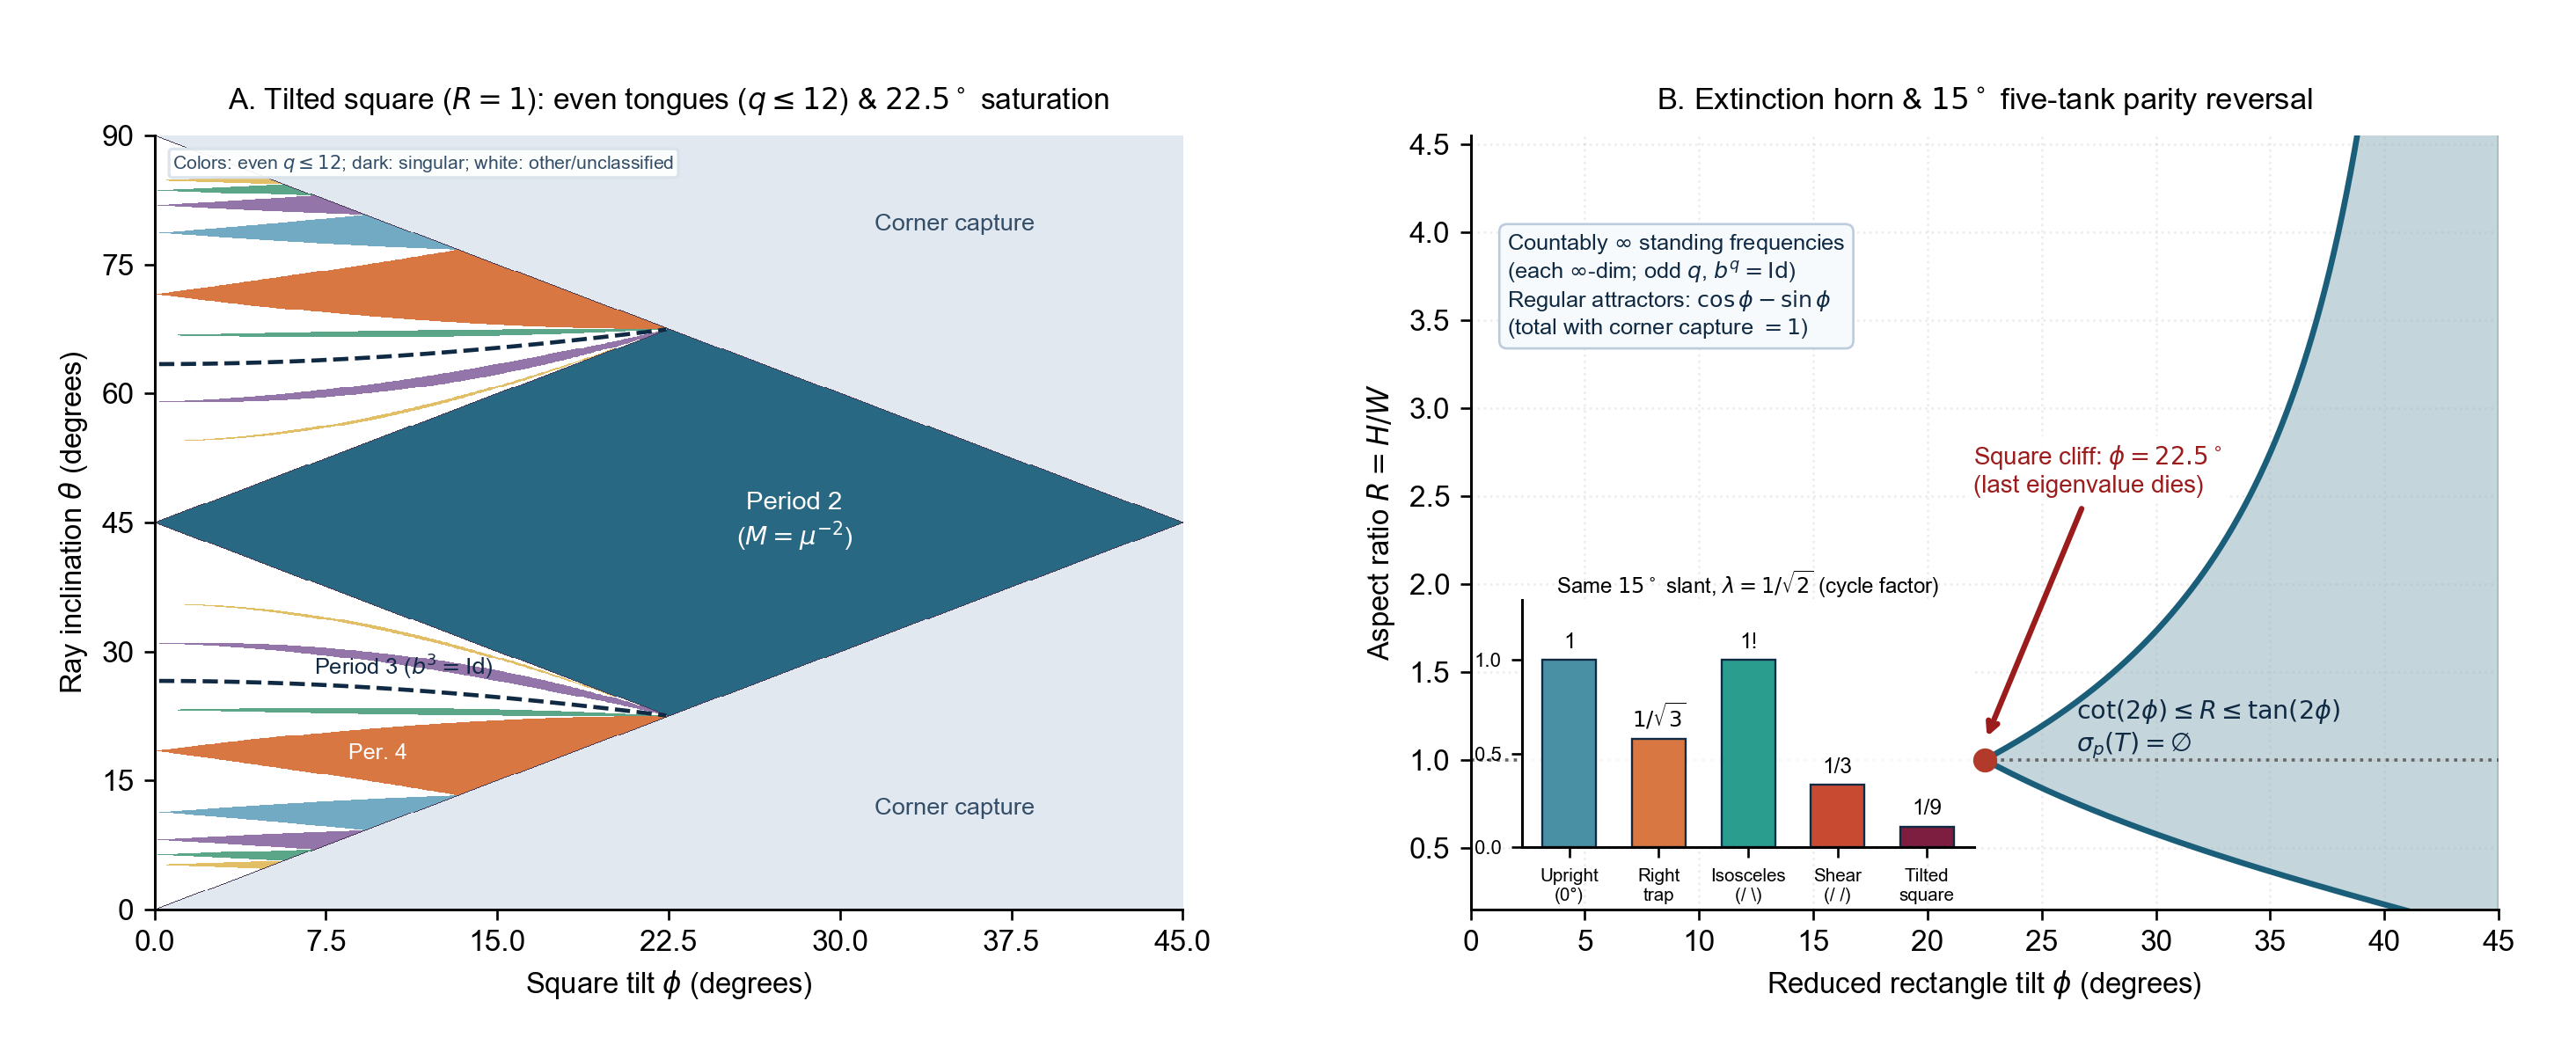
\includegraphics[width=\textwidth]{figs/p2_fig1_tilted_square_and_extinction.png}
\caption{\textbf{A.} Exact Arnold-tongue phase diagram of the tilted unit square ($R=1$), showing even-period hyperbolic tongues, corner-capture triangles, the globally neutral period-3 lines ($b^3 = \Id$), and complete saturation of the primary period-2 tongue at $\phi = 22.5^\circ$. \textbf{B.} Exact spectral extinction horn $\cot(2\phi) \le R \le \tan(2\phi)$ ($\sigma_p(T) = \varnothing$) with the square cliff at $\phi = 22.5^\circ$; inset displays the $15^\circ$ five-tank parity reversal ($1,\; 1/\sqrt{3},\; 1,\; 1/3,\; 1/9$ at $\lambda = 1/\sqrt{2}$).}
\label{fig:p2-fig1}
\end{figure}

% ==============================================================================
\section{All-Polygon Rigidity and Microscopic Corner Shaving}\label{sec:rigidity}
% ==============================================================================

We now prove that the upright rectangle is \emph{uniquely} immune to geometric wave attractors among all convex polygons, and quantify what happens when even a single corner of the unit square is shaved by a microscopic bevel.

\subsection{All-polygon rigidity and the shallow travel-time obstruction}

\begin{theorem}[All-polygon rigidity and shallow travel-time obstruction]\label{thm:rigidity}
\leavevmode
\begin{enumerate}
  \item \textbf{Global uniqueness of the upright rectangle}: Among bounded convex polygons $K \subset \R^2$, an axis-aligned rectangle is the unique shape for which every transverse physical slope $s > 0$ has neither a regular hyperbolic attracting cycle nor a one-sided attracting corner. Every other convex polygon has an open interval of transverse slopes carrying one of these two forms of attraction.
  \item \textbf{Shallow travel-time obstruction}: Suppose $K$ has positive-length horizontal top and bottom edges at $z = 0, H$ ($L(z) \le x \le R(z)$, $W(z) = R(z) - L(z) > 0$) and at least one genuine interior wall vertex at height $h \in (0, H)$. Define the travel-time coordinate
  \[
    T(y) = \int_0^y \frac{dz}{W(z)}, \qquad A = T(H), \qquad \beta_h = \frac{T(h)}{A} \in (0,1).
  \]
  There exists $C > 0$ (independent of $n$) such that for every sufficiently large integer $n$, either the one-turn resonances $s = A/n + O(n^{-3})$ contain an open interval of regular hyperbolic attracting $b_s$-cycles of primitive period $n+1$, or
  \begin{equation}\label{eq:travel-time}
    \dist(n\beta_h, \Z) \le \frac{C}{n}
  \end{equation}
  holds simultaneously at \emph{every} interior wall vertex height $h$. Consequently, at least one of every two sufficiently large consecutive integers $n, n+1$ supplies an open attracting tongue; if any $\beta_h$ is irrational, the set of attracting period labels $n$ has natural density~$1$.
\end{enumerate}
\end{theorem}

\begin{proof}
If any of the four horizontal or vertical supporting lines meets $K$ in a single vertex $v$, then for all sufficiently small (or large) transverse slopes $s > 0$, $v$ strictly extremizes both $\xi$ and $\eta$, making $v$ a fixed corner of $b_s$ with reciprocal one-sided multipliers $D, D^{-1} \ne 1$ \cite[Prop.~5]{NogueiraTroubetzkoy2020}. Conversely, on an axis-aligned rectangle the boundary metric $d\ell_s = |dz| + s|dx|$ makes both chord involutions isometries and $b_s$ a rigid rotation at every slope. If all four axial supporting faces are positive-length edges and $K$ is not an axis-aligned rectangle, then $K$ possesses at least one oblique edge, creating a genuine interior left or right wall vertex $h \in (0, H)$; Part~(1) therefore reduces to Part~(2).

To prove~(2), assume only the stated hypotheses: positive-length horizontal top and bottom edges at $z = 0, H$ and at least one genuine interior left or right wall vertex $h \in (0, H)$. Reflect $L, R$ across $z = 0, H$ to $P = 2H$-periodic piecewise-affine walls. For small $s > 0$, the ascending left-to-right and right-to-left unfolded lifts $U_s, V_s$ defined implicitly by $w - z = s[R(w) - L(z)]$ and $t - w = s[R(w) - L(t)]$ are strictly increasing in both $z$ and $s$, giving the strictly $s$-monotone left- and right-return lifts $F_s = V_s U_s$ and $G_s = U_s V_s$. One unfolded turn with $n$ left returns ($F_s^n(z) = z + P$) has $2n$ lateral wall impacts and crosses two cap lines ($z = 0, H$), giving $2n + 2$ physical impacts away from vertices and hence $n + 1$ two-chord iterates of $b_s$ (primitive period $n + 1$ since $\gcd(1, n) = 1$). For each large $n$ and each $z \bmod P$, $F_s^n(z) = z + P$ has a unique continuous solution $s_n(z) > 0$. If $s_n(z)$ is nonconstant, its open range contains slopes avoiding the finitely many vertex-resonance values $F_s^n(c) = c + P$ and $G_s^n(c) = c + P$, where the sign-changing piecewise-affine displacement $F_s^n(z) - z - P$ must have a regular downward crossing with $0 < (F_s^n)' < 1$, persisting on an open interval of $s$.

Suppose instead that $s_n(z) \equiv s$ is constant, so $F_s^n(z) = z + P$ globally. Setting $k_s(m) = (1+sm)/(1-sm)$ and differentiating both sides of the one-turn orbit yields the telescoping one-sided derivative product
\[
  1 = (F_s^n)'_\pm(z_0) = \prod_{i=0}^{n-1} \frac{k_s(R'_\pm(w_i))}{k_s(L'_\pm(z_i))}.
\]
Because $R$ is concave and $L$ is convex on every open half-period $(0, H)$ and $(H, 2H)$ while $\log k_s(m)$ increases strictly, every genuine interior wall kink contributes a \emph{strictly negative} jump to $\log (F_s^n)'_+ - \log (F_s^n)'_-$. Since the net jump must vanish, the orbit launched from any interior wall vertex $h$ must also hit a fold $0$ or $H \bmod P$! On any breakpoint-free return with local wall slopes $l = L'$ and $r = R'$, exact integration gives $T(F_s(z)) - T(z) = (\log k_s(r) - \log k_s(l))/(r - l)$ for $r \ne l$, extending continuously to $2s/(1 - s^2 r^2)$ when $r = l$ (in all cases $2s + O(s^3)$), while the boundedly many returns crossing a kink satisfy $T(F_s(z)) - T(z) = 2s + O(s^2)$. Summing over a full one-turn orbit gives $2A = 2ns + O(s^2)$, i.e., $s = A/n + O(n^{-3})$, and summing along the $m \le 2n$ half-legs between the kink at height $h$ and its fold yields $T(h) \equiv \pm m s + O(s^2) \pmod{A}$, proving \eqref{eq:travel-time}. Subtracting \eqref{eq:travel-time} for $n$ and $n+1$ would force $\dist(\beta_h, \Z) = O(1/n)$, impossible for fixed $\beta_h \in (0,1)$; when $\beta_h \notin \Q$, equidistribution of $n\beta_h \bmod 1$ yields natural density~$1$ for attracting labels.
\end{proof}

\begin{remark}[Chamfered octagon example and central period-two criterion]\label{rem:chamfer-oct}
Consider the square-symmetric chamfered octagon $K = \{|x|,|z| \le 1,\; |x|+|z| \le 3/2\}$ (Figure~\ref{fig:p2-fig2}B), which retains all four axial walls (so has zero corner capture) yet has interior sidewall vertex at $h = 1/2$ (shifted height above $z = -1$). Direct integration yields $\beta_{1/2} = \frac{\log 2}{1 + 2\log 2}$, which is irrational by the Hermite--Lindemann theorem! Thus Theorem~\ref{thm:rigidity} supplies a density-$1$ sequence of attracting period labels (e.g., exact period-3 tongue $1/2 < s < 2/3$ with $M = ((1-s)/(1+s))^2 = 1/16$ at $s = 3/5$, period-4 multiplier $121/625$ at $s = 7/18$, period-5 multiplier $36/121$ at $s = 5/17$). Yet by the following separate central criterion, this octagon admits \emph{no} regular period-two attractor at any slope.
\end{remark}

\begin{proposition}[Central symmetry period-two criterion]\label{prop:central-p2}
Let $K$ be a centrally symmetric convex polygon centered at the origin with positive axis intercepts $(a,0), (0,b)$, $r = b/a$, and $S_r(x,z) = (z/r, rx)$. Then $K$ admits a regular hyperbolic period-two cycle at some transverse slope if and only if $S_r K \ne K$. When $S_r K = K$, any transverse slope carrying a primitive period-two point must equal $r$ (such a transverse slope exists if and only if $r$ is transverse to every edge of $K$; at $s = r$, the midpoint-extended boundary map satisfies $b_r = -I$).
\end{proposition}

\begin{proof}
As in \cite[Thm.~4.3]{Paper1}, central symmetry forces every period-two orbit to take the form $(p, -q, -p, q)$ with $q = S_s p$. In the first quadrant, strict concavity of $\log x + \log z$ gives a unique maximum of $xz$ along $\partial K$, pairing each submaximal level $t = xz$ uniquely into two continuous points $p(t), q(t)$ with $q(t) = S_{s(t)}p(t)$ and $\lim_{t\downarrow 0} s(t) = r$. If $S_r K \ne K$, then $s(t)$ is nonconstant on some real-analytic edge-pair branch (up to reflecting a coordinate), so we may choose a transverse slope $s = s(t)$ with $s'(t) \ne 0$. The multiplier at $p$ is $D^2$ where $D = |g_-(e_p)g_+(e_q)/(g_-(e_q)g_+(e_p))|$ with $g_\pm(e) = e_z \pm s e_x$ for incident edge tangents $e_p, e_q$, so $D = 1$ forces either $e_q \parallel e_p$ or $e_q \parallel S_s e_p$. In a centrally symmetric polygon, two parallel edges lie on the same or opposite supporting lines, so $e_q \parallel e_p$ would place either $p, q$ or $-p, q$ on a single edge, making a characteristic parallel to that edge and contradicting transversality; meanwhile $\det(q', S_s p') = -s'(t)/s(t) \ne 0$ excludes $e_q \parallel S_s e_p$. Hence $D \ne 1$, producing an open interval of regular hyperbolic period-two cycles.

Conversely, suppose $S_r K = K$. Up to reflecting a coordinate, consider a four-impact cycle with $p, q$ in the first quadrant. If $p \ne q$ and $xz > 0$, then $S_r$ exchanges the unique pair of boundary points at that product, forcing $s = r$. If $p = q = (x, sx)$ is collapsed, the slope-$-s$ characteristic supports $K$ at $p$, so every $(x', z') \in K \cap \{x', z' \ge 0\}$ obeys $x'z' \le (z'+sx')^2/(4s) \le (2sx)^2/(4s) = xz$, making $p$ the unique product maximizer; symmetry $S_r K = K$ fixes that maximizer and again forces $s = r$. If either coordinate vanishes, the axis intercepts force $s = r$ directly. Finally, $S_r$ and $-S_r$ preserve $\xi$ and $\eta$ chords respectively ($\xi \circ S_r = \xi$, $\eta \circ (-S_r) = \eta$), giving $b_r = -I$ (with midpoint reflection on any characteristic edge).
\end{proof}

\subsection{Microscopic corner shaving: permanent \texorpdfstring{$17.80577\%$}{17.80577 percent} frequency collapse}
What happens quantitatively when we break the upright square's rigidity by removing a single microscopic corner triangle?

\begin{theorem}[Microscopic corner shaving and permanent measure jump]\label{thm:shaving}
Let $\Omega_{u,v}$ be the axis-aligned unit square $[0,1]^2$ with its northeast corner removed by a straight bevel of horizontal leg $u$ and vertical leg $v$ ($0 < u \le v < 1$, bevel slope ratio $\tau = v/u \ge 1$).
\begin{enumerate}
  \item \textbf{Five-sided rigidity}: For any axis-aligned $W\times H$ rectangle with a proper straight corner cut joining the relative interiors of two adjacent sides, there is an open interval of transverse slopes with a regular period-three attractor. In normalized unit-square coordinates (normalized slope $sW/H$ and relative cut legs $0 < u \le v \le 1/2$), the exact set of \emph{shallow} slopes $0 < s < 1$ carrying a regular hyperbolic period-three attractor is precisely $1/2 < s < 1/(2-u)$ (with a symmetric steep window above $s = 1$ when diagonal reflection applies). Alignment is essential: the cut tilted diamond $\{|x|+|z| \le 1,\; z \le 1/2\}$ has a fixed corner trap at every transverse slope and no period-three tongue.
  \item \textbf{Exact rational plateaus (Theorem~4b)}: Let $1 \le m < n$ be coprime and set $s_* = m/(n-u)$. Whenever $s_* < \tau$ and $v + s_* u < 1/n$, the complete right-return rotation-$m/n$ plateau in $0 < s < \tau$ is the exact closed interval $[m/n,\, m/(n-u)]$. At the lower endpoint $s = m/n$, $\ker(T - \lambda^2)$ is infinite dimensional; throughout $(m/n,\, m/(n-u)]$, $\ker(T - \lambda^2) = \{0\}$; and at every interior slope $s \in (m/n,\, m/(n-u))$ there is a unique regular $2(m+n)$-bounce attracting ray with exact, $u$-independent full-cycle multiplier $(\tau - s)/(\tau + s)$.
  \item \textbf{Permanent limiting frequency measure (Corollary~4c)}: For equal cut legs $u = v = \varepsilon \downarrow 0$ (removed area $\varepsilon^2/2 \to 0$), let $\mathcal{A}_\varepsilon \subset (0,1)$ be the set of physical frequencies $\lambda$ carrying a regular hyperbolic attractor and zero Dirichlet kernel. Then
  \begin{equation}\label{eq:shaving-jump}
    \liminf_{\varepsilon \downarrow 0} |\mathcal{A}_\varepsilon|_\lambda \ge \frac{6}{\pi^2}\left(1 - \frac{1}{\sqrt{2}}\right) = 0.1780577256659594\ldots,
  \end{equation}
  while the limiting angular-fraction lower bound on $(0,\pi/2)$ is
  \[
    \frac{12}{\pi^3}\left(\frac{\pi}{4} - \frac{1}{2}\log 2\right) = 0.1698331899603879\ldots,
  \]
  and the bevel-midpoint period-three multiplier $(2-\varepsilon)/(6-\varepsilon)$ (attained at bevel midpoint $h = \varepsilon/2$, slope $s = 1/(2-\varepsilon/2)$) stays bounded away from $1$ and tends to $1/3$.
\end{enumerate}
\end{theorem}

\begin{proof}
(\emph{Part 1}) Rescaling the $W\times H$ rectangle to $[0,1]^2$, reflecting the bevel to the northeast corner, and exchanging axes so $0 < u \le v < 1$ ($\tau = v/u \ge 1$) preserves the family of opposite-slope ray pairs. Unfolding only horizontal and vertical walls replaces the omitted corners by open diamonds $|X-(2i+1)|/u + |Z-(2j+1)|/v < 1$. For small $h > 0$, set $p = u(1 - h/v)$ and $s = 1/(2-p) < 1 \le \tau$, and join $A = (1-p, 1-h)$ to $A' = (-3+p, -1-h)$. Because $1/u > s/v$, the weighted distance along $AA'$ to every diamond center in a given column is minimized at its column abscissa; in the single intermediate column $X = -1$ the ordinate is $-h$ (at vertical distance $1 - h > v$ from centers), while the vertical grid crossings $X = 0, -1, -2$ lie at ordinates $s-h, -h, -s-h$, avoiding integer heights for small $h$. Thus $AA'$ folds to a regular 6-reflection (period-3) closed ray. Varying $p$ at fixed $s$ gives $(\tau - s)p' = (\tau + s)p + 2 - 4s$, yielding repelling multiplier $(\tau+s)/(\tau-s)$ and time-reversed attracting multiplier $(\tau-s)/(\tau+s)$ on an open interval of $s$.

When $0 < u \le v \le 1/2$, every $h \in (0, v)$ satisfies $h < 1 - v$, $h < s$, and $h + s(h) < v + 1/2 \le 1$, proving sufficiency across $1/2 < s < 1/(2-u)$. Conversely, for $0 < s < 1 \le \tau$, any regular period-3 orbit reflects horizontally off the bevel and makes $m$ vertical and $n$ horizontal round trips with $m + n = 3$ and $m/s = \sum_{j=1}^n W(z_j) \le n$, forcing $m = 1, n = 2$, $s(W(z_1) + W(z_2)) = 1$, and $z_2 = 1 - z_1$. Because the bevel lies in $z > 1 - v \ge 1/2$, at most one right impact hits it: zero hits forces $s = 1/2$, whereas one regular hit forces $2 - u < 1/s < 2$, i.e., $1/2 < s < 1/(2-u)$, and excludes multiplier $1$ (hence any neutral periodic interval). On the cut diamond $\{|x|+|z| \le 1,\; z \le 1/2\}$, $(0,-1)$ strictly minimizes both $\xi$ and $\eta$ for $0 < s < 1$ while $(1,0)$ strictly maximizes $\xi$ and minimizes $\eta$ for $s > 1$; every transverse slope therefore has a fixed corner trap and rotation $0$, ruling out any period-three tongue.

(\emph{Part 2}) For $0 < s < \tau$, the bevel reverses horizontal velocity like a vertical wall, and the right-wall abscissa $W(t)$ in the $2$-periodic unfolded vertical coordinate $t$ equals $1$ except on $\{|t - 1| < v\}$, where $W(t) = 1 - u + (u/v)|t - 1|$. The physical right-return lift $T_s$ defined implicitly by $T_s(t) - t = s[W(t) + W(T_s(t))]$ is continuous and strictly increasing in $s$ (hence has nondecreasing rotation number). Introducing the shifted phase $y = t - s W(t)$ and deficit tent $d(y) = 1 - W(t) \in [0, u]$---supported on $B = [1-s-v,\, 1-s+v]$ of length $2v$ with apex at $1 - s(1-u)$---converts the right-return lift into
\[
  S_s(y) = y + 2s - 2s\,d(y).
\]
Along any $n$-periodic orbit of winding $m$, the total deficit is $D = \sum_{j=0}^{n-1} d(y_j) = n - m/s$. For any partial block of $0 < k < n$ steps with deficit $D_k \in [0, D]$, the displacement differs from $2km/n$ by $2s(kD/n - D_k)$, whose magnitude is at most $2sD$. Because $\gcd(m,n) = 1$, distinct visits on the circle of circumference $2$ are separated by at least $2/n - 2sD$. Under $v + s_* u < 1/n$, every $s \in [m/n, s_*]$ gives $0 \le D \le u$ and $2/n - 2sD > 2v$, forcing \emph{at most one} orbit point to enter $B$!

For $0 < D < u$, the tent $d(y) = D$ has exactly two preimages $y_0^\pm$ on the two affine branches of $B$. Launching from either yields the candidate iterates $y_k = y_0 + 2ks - 2sD$ ($1 \le k \le n$), which return to $y_0 + 2m$ at $k = n$ and satisfy $|y_k - y_0| \ge 2/n - 2sD > 2v$ modulo $2$ for $1 \le k < n$, proving they stay outside $B$ and form an exact $n$-periodic orbit with derivatives $(1 \pm s/\tau)/(1 \mp s/\tau)$ at the unique bevel hit and derivative $1$ at all $n-1$ axial hits, giving reciprocal full-cycle multipliers $(\tau - s)/(\tau + s)$ and $(\tau + s)/(\tau - s)$. Passing through an axial $90^\circ$ corner would equate the directed ray with its reverse, contradicting the opposite vertical velocities at the bevel; hence both orbits are regular and exclude any neutral periodic interval. At $D = 0$ ($s = m/n$), $2nv < 2$ leaves an open arc of bevel-free regular neutral rays (yielding infinite-dimensional modes); at $D = u$ ($s = s_*$), the unique apex preimage gives a corner cycle with no periodic interval. For $s < m/n$, every step obeys $S_s(y) - y \le 2s$, so the rotation number is strictly below $m/n$. Just above $s_*$, $D > u$ while $2/n - 2sD > 2v$ persists, making a single-visit deficit $> u$ impossible; strict monotonicity of $T_s$ in $s$ then globally excludes rotation $m/n$ for all $s > s_*$.

(\emph{Part 3}) Set $u = v = \varepsilon$ ($\tau = 1$) and $N = \lfloor 1/\varepsilon \rfloor - 1$. Every coprime pair $1 \le m < n$ with $m + n \le N$ satisfies $s_* = m/(n-\varepsilon) < 1$ and $n\varepsilon(1 + s_*) = \varepsilon(m+n) + m\varepsilon^2/(n-\varepsilon) < 1$, certifying disjoint open attracting plateaus $(m/n,\, m/(n-\varepsilon))$ of slope length $\varepsilon(m/n)/(n-\varepsilon)$ (e.g., $39{,}797$ disjoint plateaus below $s=1$ at $\varepsilon = 1/512$; Figure~\ref{fig:p2-fig2}A). Diagonal symmetry $s \leftrightarrow 1/s$ adds their reciprocal plateaus above $s = 1$, giving combined frequency-density weight $g_\lambda(x) = (1+x)/(1+x^2)^{3/2}$ on $x = m/n \in (0,1)$ (and $g_\theta(x) = 2/(1+x^2)$ for angle). Rescaling $(m,n) = N(a,b)$ on $\{0 < a < b,\; a+b \le 1\}$, where primitive lattice points have density $1/\zeta(2) = 6/\pi^2$ by M\"obius inversion and the small-$n$ boundary strip $n < \delta N$ contributes $O(\delta)$ uniformly in $N$, evaluates the limiting Riemann sum as
\[
  \frac{6}{\pi^2}\int_0^1 \frac{x}{1+x}\,g_\lambda(x)\,dx = \frac{6}{\pi^2}\int_0^1 \frac{x}{(1+x^2)^{3/2}}\,dx = \frac{6}{\pi^2}\left(1 - \frac{1}{\sqrt{2}}\right),
\]
where the factor $(1+x)$ cancels identically! For the angular fraction on $(0,\pi/2)$ (dividing by $\pi/2$), $\frac{2}{\pi}\cdot\frac{6}{\pi^2}\int_0^1 \frac{x}{1+x}\frac{2}{1+x^2}\,dx = \frac{12}{\pi^3}(\frac{\pi}{4} - \frac{1}{2}\log 2)$.
\end{proof}

\begin{figure}[ht]
\centering
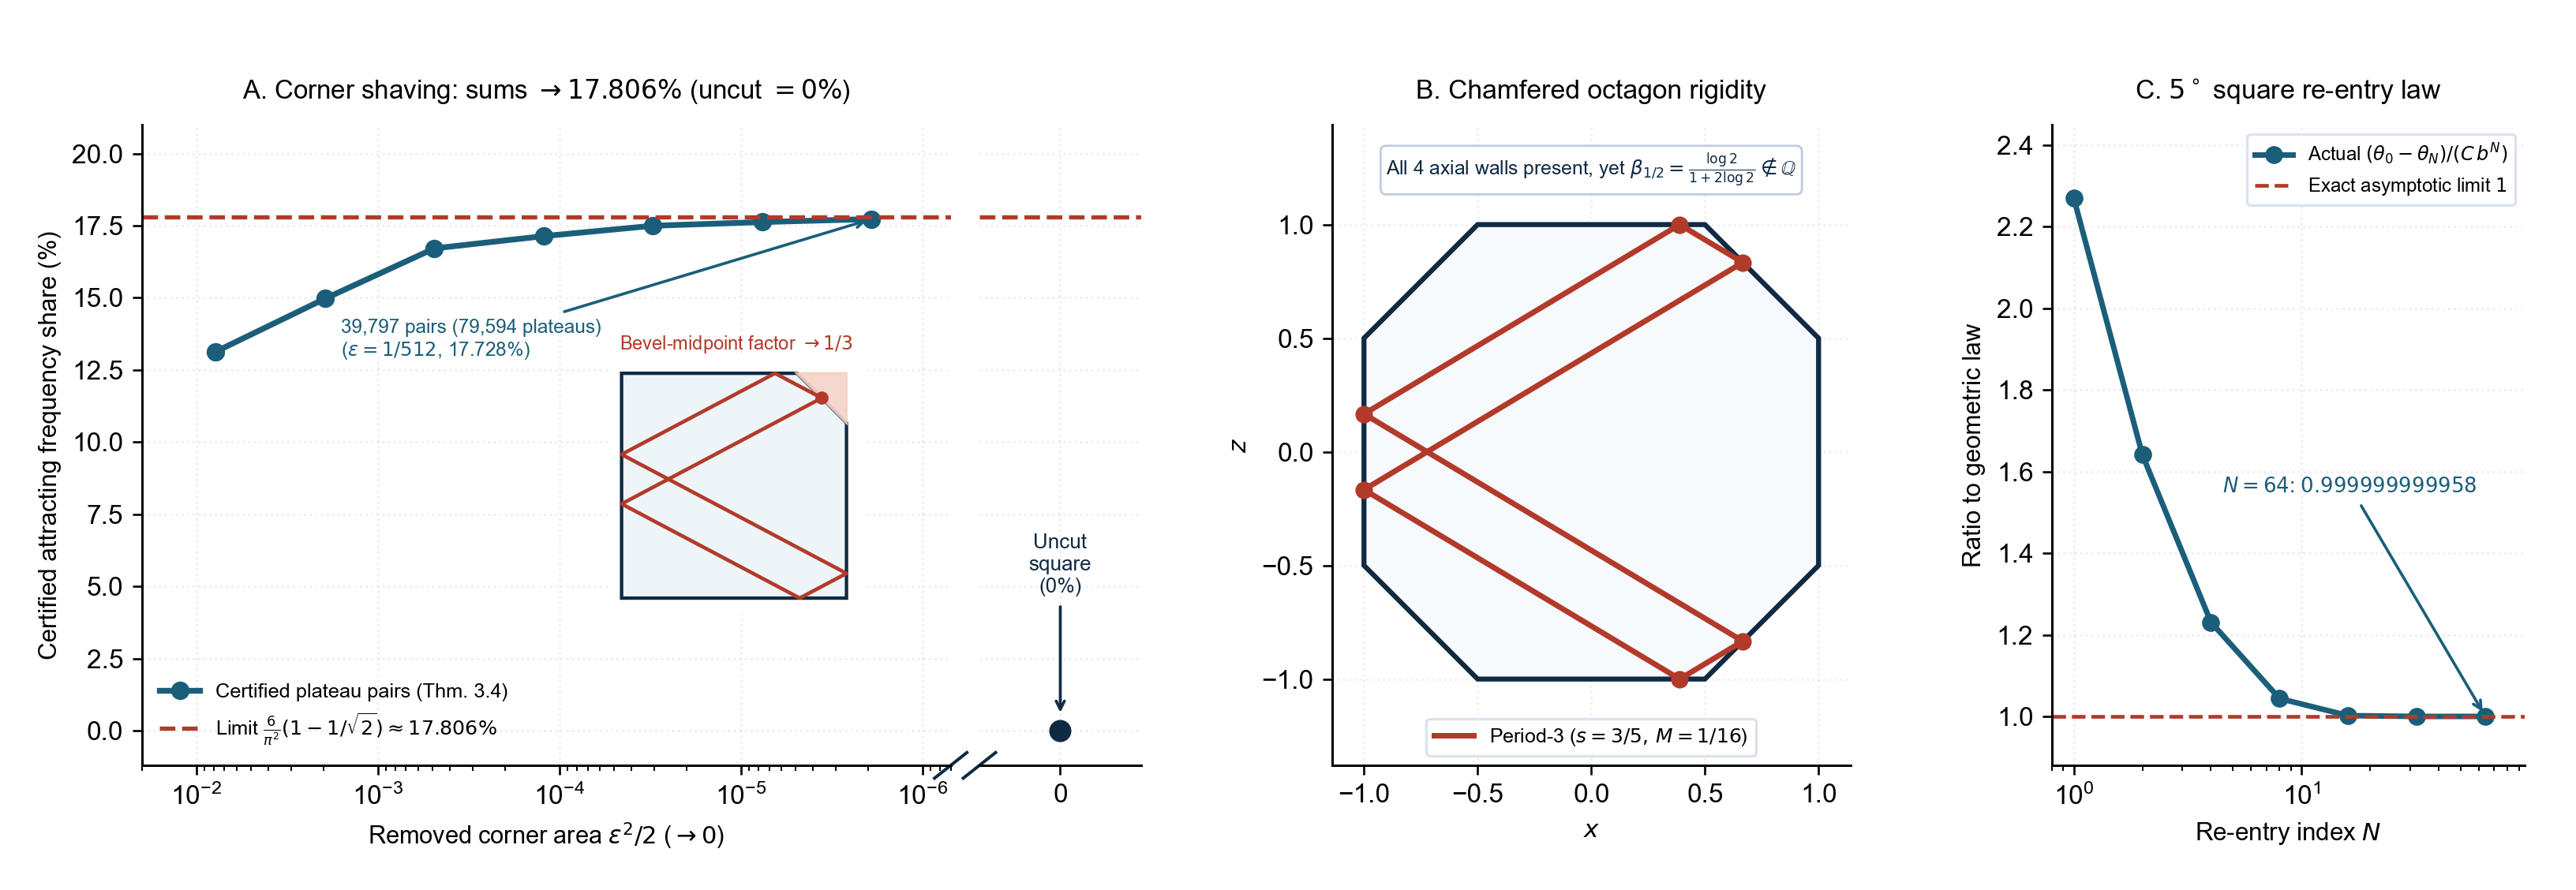
\includegraphics[width=\textwidth]{figs/p2_fig2_shaving_and_rigidity.png}
\caption{\textbf{A.} Microscopic corner shaving on the unit square (Theorem~\ref{thm:shaving}): for dyadic cuts $\varepsilon = 2^{-k}$ ($3 \le k \le 9$, removed corner area $\varepsilon^2/2 \to 0$), the certified disjoint-plateau sums approach the universal limiting floor $C = \frac{6}{\pi^2}(1 - 1/\sqrt{2}) = 17.80577\ldots\%$ (reaching $17.728\%$ from $39{,}797$ reciprocal pairs, i.e., $79{,}594$ intervals, at $\varepsilon = 1/512$; bevel-midpoint factor $(2-\varepsilon)/(6-\varepsilon) \to 1/3$), proving $\liminf_{\varepsilon\downarrow 0}|\mathcal{A}_\varepsilon|_\lambda \ge C$ despite $0\%$ on the uncut square. \textbf{B.} Square-symmetric chamfered octagon retaining all four axial walls yet possessing irrational travel-time ratio $\beta_{1/2} = \log 2/(1+2\log 2)$ and exact period-3 attractor ($M = 1/16$ at $s = 3/5$). \textbf{C.} Live 95-digit verification of the geometric re-entry law \eqref{eq:reentry} on the $5^\circ$ tilted square, normalized by $C b^N$ with $C = t_0/(1+Rt_0)$ and $b = (R-t_0)/(R(1+Rt_0))$ ($t_0 = \tan 2\phi$; ratio $0.999999999958$ at $N = 64$).}
\label{fig:p2-fig2}
\end{figure}

% ==============================================================================
\section{Regular \texorpdfstring{$N$}{N}-Gons and the Disk-Limit Paradox}\label{sec:regular}
% ==============================================================================

We now study the unit-circumradius regular $N$-gon $P_N(\phi)$ with vertices at angles $\phi + 2jh$ ($h = \pi/N$), satisfying $d_H(\partial P_N(\phi), \partial D) = d_H(\overline{P_N(\phi)}, \overline{D}) = 1 - \cos(\pi/N) \to 0$ as $N \to \infty$ (where $D$ is the unit disk). On the disk, $b_\lambda$ is a rigid clockwise rotation by $4\theta$ ($\rho_{\mathrm{CW}} = 2\theta/\pi$) and polynomial eigenfunctions form a complete basis \cite{Aleksandryan1960}. Yet regular polygons display an astonishing mix of exact disk-frequency survival, mod-$4$ corner trapping, discontinuous zero-tilt Lyapunov cliffs, and persistent $O(1)$ contraction at the half-frequency $\lambda = 1/\sqrt{2}$.

\subsection{Exact \texorpdfstring{mod-$4$}{mod-4} corner capture and uniform disk shadowing}

\begin{theorem}[Mod-$4$ corner-capture fractions and uniform shadowing]\label{thm:corner-shadow}
Set $h = \pi/N$ and $d(t) = \dist(t,\, \phi + 2h\Z + \pi\Z)$, with $A = h - d(\pi/2)$ and $B = h - d(0)$.
\begin{enumerate}
  \item Away from the finitely many characteristic angles, the boundary map $b_\lambda$ has clockwise rotation number $0 \pmod 1$ (common supporting corner) precisely on $0 < \theta < A$ and $\pi/2 - B < \theta < \pi/2$. The exact angular fraction $2(A+B)/\pi$ and physical frequency measure $1 - \cos A + \sin B$ obey
  \begin{equation}\label{eq:mod4-corner}
    \text{angular corner fraction} =
    \begin{cases}
      3/N, & N \text{ odd } (N \ge 5;\; 1 \text{ for } N=3), \\
      2/N, & N \equiv 2 \pmod 4, \\
      (4/N)(1 - d(0)/h), & 4 \mid N.
    \end{cases}
  \end{equation}
  In particular, face-normal aligned $N = 4m+2$ polygons ($\phi \equiv h \pmod{2h}$, where $B = 0$ and $A = h$) have quadratically decaying frequency corner measure $1 - \cos(\pi/N) \sim \pi^2/(2N^2)$ (whereas vertex alignment $\phi = 0$ gives $A = 0, B = h$ and linear frequency corner measure $\sin(\pi/N)$), while $4\mid N$ polygons with horizontal and vertical edges have zero corner measure.
  \item Every noncritical angle obeys the uniform disk-shadowing bound $|\rho_{\mathrm{CW}}(b_\lambda) - 2\theta/\pi| \le 2/N$ (established via the continuous clockwise lift $F_\theta$ of $b_\lambda$ in polar angle).
\end{enumerate}
\end{theorem}

\begin{proof}
A fixed point of $b_\lambda$ is fixed by both chord involutions, which holds iff both characteristic normals lie in the normal cone (half-width $h$) of a single vertex; matching the two projective normal-circle bisectors at $0$ and $\pi/2$ yields $\theta < A$ and $\pi/2 - \theta < B$. Modulo $\pi$, the projective vertex grid has spacing $h$ for odd $N$ (with $0$ and $\pi/2$ half a grid spacing apart, so $d(0) + d(\pi/2) = h/2$), spacing $2h$ for $N \equiv 2 \pmod 4$ (with $d(0) + d(\pi/2) = h$), and $d(0) = d(\pi/2)$ for $4 \mid N$, yielding \eqref{eq:mod4-corner} immediately (Figure~\ref{fig:p2-fig3}C; formally verified in Lean~4 by \texttt{regular\_corner\_fractions}). For~(2), since $|\partial_t \log r(t)| \le \tan h$, any chord between angles $a \pm D$ ($0 < D \le \pi/2$) deviates from the disk tangent at $a$ by angle $e$ satisfying $|\tan e| = \frac{|r_2 - r_1|}{r_2 + r_1}\cot D \le \frac{1}{2}|\log r_2 - \log r_1|\cot D \le D\tan h\cot D \le \tan h$, so each chord shifts the endpoint angle by at most $2h$ from the disk reflection; composing the continuous chord lifts gives $|F_\theta(t) - (t - 4\theta)| \le 4h$ for the continuous clockwise lift $F_\theta$, and hence $|\rho_{\mathrm{CW}}(b_\lambda) - 2\theta/\pi| \le 2/N$.
\end{proof}

\subsection{The resonance grid, exact eigenfrequency survival, and the half-frequency paradox}

\begin{theorem}[Resonance grid, telescoping product, and exact eigenfrequency survival]\label{thm:res-grid}
\leavevmode
\begin{enumerate}
  \item \textbf{Resonance grid}: Set $\theta = k\pi/(2N)$ with $1 \le k < N$, $g = \gcd(k, N)$, $k/N = p/q$ in lowest terms, and $\eta = \pi/2 + \theta$. Whenever $\eta \notin \phi + h\Z$ (so no wall is characteristic and all grid impacts lie in edge interiors), the rays $t_j = \eta + jh$ ($j \bmod 2N$) carry $2g - 2$ regular period-$q$ cycles. For odd $q$ and $g \ge 2$, each of the $2g - 2 \ge 2$ cycles lies in an open neutral interval fixed by $b^q$ (yielding infinite-dimensional eigenmodes). For even $q = 2r$, exactly $g - 1$ cycles attract and $g - 1$ repel, with full-period attracting multipliers and telescoping product
  \begin{equation}\label{eq:grid-mult}
    M_j = \left[\frac{\tan(r(jh - d_j))}{\tan(r(jh + d_j))}\right]^2 \quad (1 \le j < g), \qquad
    \prod_{j=1}^{g-1} M_j = [\tan(r d_0)\tan(r d_g)]^2,
  \end{equation}
  where $d_j = |\delta_j| \in (0, h)$ is the unsigned angle between $t_j$ and its edge outward normal ($\delta_j$ the signed angular offset, $d_j + d_{j+1} = h$).
  \item \textbf{Exact disk eigenfrequency survival}: Every rational disk eigenfrequency $\theta = \pi p/(2q)$ ($0 < p < q$) survives \emph{exactly}, with infinite multiplicity, on every vertex-aligned ($\phi = 0$) regular $N = 4mq$-gon ($m \ge 1$). In particular, at $E = 1/2$ ($\theta = \pi/4$), every aligned regular polygon with $8 \mid N$ (e.g., $N = 1000$) satisfies $b^2 = \Id$ globally and has $\dim \ker(T_N - 1/2) = \infty$.
\end{enumerate}
\end{theorem}

\begin{proof}
Reflecting $t_j$ across $\eta$ and then across $\eta - kh = \pi/2 - \theta$ preserves the polygonal radius $r(t)$ (period $2h$) and maps $t_j \mapsto t_{j-2k}$. Removing the two degenerate cycles containing $j \equiv 0, k \pmod N$ leaves $2g - 2$ regular cycles of period $q$. Evaluating the boundary-length derivative along each cycle gives $(b^q)'(t_j) = \prod_{\ell=0}^{q-1} A(j - 2k\ell)/A(j - (2\ell+1)k)$ with $A(u) = |\sin(uh+\delta_j)/\sin(uh-\delta_j)|$, where $\delta_j \in (-h, h) \setminus \{0\}$ is the signed angular offset from $t_j$ to its edge outward normal ($d_j = |\delta_j|$). For odd $q$, doubling permutes residues modulo $q$ and cancels all factors to $1$; for even $q = 2r$, the identity $\prod_{\ell=0}^{r-1}|\sin(x + \ell\pi/r)| = 2^{1-r}|\sin(rx)|$ yields \eqref{eq:grid-mult}, and $d_j + d_{j+1} = h$ telescopes the product. For~(2), when $N = 4mq$ and $\phi = 0$, both normal directions $\pi/2 \pm \theta$ are opposite-vertex mirror axes of $P_N(0)$, so $b$ is a rigid rotation by $-2\pi p/q$ with $b^q = \Id$ globally and no characteristic walls, ensuring that $\ker(T_N - \lambda^2)$ contains an infinite-dimensional subspace of $C^\infty$ modes by \cite[Thm.~2.2]{Paper1}. (Note that on aligned $8 \mid N$ polygons at $E = 1/2$, $\ker(T_N - 1/2)$ contains an infinite-dimensional subspace of smooth $b^2$-invariant waves, \emph{not} the literal disk polynomial $1 - x^2 - z^2$, which has nonzero trace $\sin^2(\pi/N) > 0$ at face midpoints.)
\end{proof}

Compare $N = 1000$ ($8 \mid N$, infinite-dimensional exact eigenspace at $E = 1/2$) with $N = 1002$ ($N = 4m+2$): adding just two sides shatters the entire eigenspace into $500$ wave attractors while leaving behind a near-perfect spectral ghost!

\begin{theorem}[The Half-Frequency Paradox and Quantitative Ghost Quasimode]\label{thm:half-freq-paradox}
Consider the vertex-aligned ($\phi = 0$) regular polygon $P_N(0)$ with $N = 4m + 2$ ($m \ge 1$, $L = N/2 - 1 = 2m$) at $\lambda = 1/\sqrt{2}$ ($E = 1/2$, $s = 1$).
\begin{enumerate}
  \item \textbf{500 attractors and pinned $1/3$ contraction}: $\ker(T_N - 1/2) = \{0\}$, and the complete periodic set consists of exactly $L = N/2 - 1$ attracting and $L$ repelling period-two cycles, with per-step contraction factors
  \begin{equation}\label{eq:half-freq-factors}
    m_j = \frac{\sin(2jh) - \sin h}{\sin(2jh) + \sin h} \qquad (1 \le j \le L,\;\; h = \pi/N).
  \end{equation}
  As $N \to \infty$, the strongest per-step contraction factor stays strictly below $1/3$ and converges to $1/3$:
  \[
    m_{\min} = \frac{2\cos(\pi/N) - 1}{2\cos(\pi/N) + 1} \uparrow \frac{1}{3} \qquad (\text{at } N=1002:\; L=500,\;\; m_{\min} = 0.33333115).
  \]
  For a ray launched uniformly in boundary arclength with asymptotic per-step log-contraction $\ell_N$,
  \begin{equation}\label{eq:arcsine-law}
    \mathbb{E}[\ell_N] = \frac{2\log\tan(h/2) + \log m_{\min}}{N/2} \sim -\frac{4\log(2N/\pi)}{N}, \qquad
    -N\ell_N \Longrightarrow \frac{2\pi}{\sin(\pi U)}, \quad U \sim \mathrm{Unif}(0,1),
  \end{equation}
  with the median of $-\ell_N$ asymptotic to $2\sqrt{2}\pi/N$ and heavy tail $\mathbb{P}(-N\ell_N \ge y) \to \frac{2}{\pi}\arcsin(2\pi/y) \sim 4/y$ for $y \ge 2\pi$ (and limiting probability $1$ for $y < 2\pi$).
  \item \textbf{Quantitative $O(N^{-3/2})$ ghost quasimode}: Despite $\ker(T_N - 1/2) = \{0\}$ and $N/2 - 1$ attractors, the explicit Dirichlet-adjusted disk polynomial $w_N(r,t) = (1 - r^2) - (1 - R_N(t)^2)(r/R_N(t))^N \in H_0^1(P_N)$ satisfies
  \begin{equation}\label{eq:quasimode}
    \frac{\|(T_N - \tfrac{1}{2})w_N\|_{H_0^1}}{\|w_N\|_{H_0^1}} \le \frac{D_N}{2(a_N^2 - D_N)} = O(N^{-3/2}),
  \end{equation}
  where $a_N = \cos h$ and $D_N^2 = \frac{1}{2N}[N^2\sin^4 h + (2 + (N-2)\sin^2 h)^2 \tan^2 h]$. At $N = 1002$, this relative residual upper bound equals $0.000130638$, concentrating all but $O_\delta(N^{-3})$ of its spectral measure within distance $\delta$ of $E = 1/2$.
\end{enumerate}
\end{theorem}

\begin{proof}
(\emph{Part 1}) By Proposition~\ref{prop:central-p2}, every period-two orbit at $s = 1$ satisfies $b(p) = -p$ with intermediate point $-S_1 p$ (coordinate swap), so regular orbits correspond exhaustively to intersections of $\partial P_N(0)$ with its $45^\circ$-reflection avoiding the four grazing rays $\pi/4 \bmod \pi/2$, which are precisely the $2N - 4$ grid rays $t_j = \pi/4 + jh$ giving the $L = N/2 - 1$ attracting and repelling cycles of Theorem~\ref{thm:res-grid} with $r = 1$, $d_j = h/2$, yielding \eqref{eq:half-freq-factors}. Finiteness of $\Fix(b^2)$ forces $\ker(T_N - 1/2) = \{0\}$ by \cite[Thm.~2.2]{Paper1}. On the antipodal quotient (perimeter $N/2$ edges), the $L$ attracting points alternate with $L$ repellers; every interior basin spans exactly one edge length while the two basins bordering the omitted grazing rays ($j=1$ and $j=L$, both having factor $m_{\min}$) jointly absorb one extra edge length, yielding the exact mean in \eqref{eq:arcsine-law} via the telescoping product \eqref{eq:grid-mult}. For any $\delta \in (0, 1/2)$, on the interior band $\delta \le u_j = 2j/N \le 1 - \delta$ we have the uniform bulk asymptotic $-N\log m_j = 2\pi/\sin(\pi u_j) + o_\delta(1)$, while the excluded endpoint basins carry total arclength mass $O(\delta + 1/N)$; letting $N \to \infty$ and then $\delta \downarrow 0$ yields the weak limit \eqref{eq:arcsine-law} (Figure~\ref{fig:p2-fig3}A).

(\emph{Part 2}) Writing $E_N(r,t) = g(t)(r/R_N(t))^N$ with $g(t) = 1 - R_N(t)^2$, we have $w_N \in H_0^1(P_N)$ since $E_N|_{\partial P_N} = g = (1-r^2)|_{\partial P_N}$ and $r^N$ smooths the origin. Because $u = 1 - x^2 - z^2$ solves $u_{zz} - u_{xx} = 0$, integration by parts against any $v \in H_0^1(P_N)$ gives
\[
  |\langle (T_N - \tfrac{1}{2})w_N, v \rangle_{H_0^1}| = \tfrac{1}{2}\left|\int_{P_N} (\partial_x E_N\,\partial_x \bar v - \partial_z E_N\,\partial_z \bar v)\,dx\,dz\right| \le \tfrac{1}{2}\|\nabla E_N\|_{L^2}\|\nabla v\|_{L^2}.
\]
Integrating $|\nabla E_N|^2$ analytically in $r \in [0, R_N(t)]$ using $g' = -2R_N^2(\log R_N)'$ yields $\|\nabla E_N\|_{L^2}^2 = \frac{1}{2N}\int_0^{2\pi} [N^2 g^2 + (2 + (N-2)g)^2 ((\log R_N)')^2]\,dt \le 2\pi D_N^2$, while the incircle gives $\|\nabla u\|_{L^2(P_N)} \ge \sqrt{2\pi}\,a_N^2$. By the triangle inequality, $\|w_N\|_{H_0^1} \ge \sqrt{2\pi}(a_N^2 - D_N)$, proving \eqref{eq:quasimode} (since $D_N = O(N^{-3/2})$).
\end{proof}

\begin{proposition}[Regular octagon zero-tilt Lyapunov cliff and \texorpdfstring{$4\mid N$}{4|N} half-period tongues]\label{prop:octagon-cliff}
\leavevmode
\begin{enumerate}
  \item At $\lambda = 1/\sqrt{2}$ ($s = 1$), the vertex-up regular octagon ($\phi = 0$) has all edges transverse to $\pm 45^\circ$ and satisfies $b^2 = \Id$ ($\Lambda = 0$ everywhere). Tilting by any small angle $\phi \in (0, \pi/8)$ shatters neutrality into three attracting period-two cycles: two exponents vanish continuously as $\phi \downarrow 0$, while the middle cycle ($j = 2$, covering $1/4$ of the boundary in polar angle) has exponent $\Lambda_2(\phi) = \log[\tan(\pi/8 + \phi)/\tan(3\pi/8 - \phi)]$, jumping discontinuously as $\phi \downarrow 0$ to
  \[
    \lim_{\phi \downarrow 0} \Lambda_2(\phi) = \log\frac{\tan(\pi/8)}{\tan(3\pi/8)} = -2\log(1 + \sqrt{2}) = -1.7627471740\ldots
  \]
  (per-step contraction factor $3 - 2\sqrt{2} = 0.171573\ldots$; Figure~\ref{fig:p2-fig3}B).
  \item For every $4 \mid N$ and any vertex phase $\phi$, letting $\epsilon = \dist(\pi/4,\, \phi + h\Z) \le \pi/(2N)$, the complete open half-rotation tongue is precisely $\pi/4 - \epsilon < \theta < \pi/4 + \epsilon$ (angular width $2\epsilon$, frequency length $\sqrt{2}\sin\epsilon$).
\end{enumerate}
\end{proposition}

\begin{proof}
Part~(1) follows immediately from evaluating Theorem~\ref{thm:res-grid} at $N = 8$, $r = 1$: the $j = 2$ attracting points lie on the horizontal axis with offset $\varepsilon_2 = \phi - \pi/8 \to -\pi/8$ as $\phi \downarrow 0$ (impacts approaching four vertices of the untilted octagon), flanked by the neighboring repellers on $(-\pi/8, \pi/8)$ and $(7\pi/8, 9\pi/8)$, which bound a total polar-angle basin of $\pi/2$ ($1/4$ of the circle).

For~(2), quarter-turn symmetry makes $xz$ on the first-quadrant boundary achieve its unique maximum at a point determined by a mirror axis $\beta$ nearest $\pi/4$: if $\beta$ is a vertex direction, that vertex maximizes $xz$ (slope $\tan\beta$), whereas if $\beta$ is a face-normal direction, the boundary point of radial angle $\pi/2 - \beta$ maximizes $xz$ (slope $\cot\beta$); at a tie $\epsilon = h/2$, both endpoints are characteristic. Continuity across the level sets of $xz$ (together with quarter-turn reflection $s \leftrightarrow 1/s$) yields half-rotation orbits throughout the open band $(\pi/4 - \epsilon, \pi/4 + \epsilon)$. To exclude half-rotation strictly outside $[\pi/4 - \epsilon, \pi/4 + \epsilon]$, extend chord maps by midpoint reflection on characteristic edges solely to compare lifts across critical angles; as $\theta$ increases, the two chord directions turn in opposite senses and the second chord map reverses boundary orientation, so $b_\theta$ and $Cb_\theta$ admit pointwise-ordered lifts with monotone rotation number throughout $(0, \pi/2)$ (note that a supporting vertex may remain fixed over an angle interval, so strict pointwise monotonicity need not hold everywhere). At any positive-width endpoint ($\epsilon > 0$), at least one chord involution is reflection in a polygon symmetry axis $L$; up to reversing flights, a half-period orbit must satisfy $p' = -p$ followed by a supporting second flight, leaving only the two antipodal radial points along the perpendicular diameter $L^\perp$ (the first-flight direction). At a unique nearest vertex-axis mirror ($0 < \epsilon < h/2$), the sole candidate zeros of $Cb_\theta$ are those two antipodal vertices, and the displacement of $Cb_\theta$ has one constant sign on both complementary arcs (while taking both signs at $\theta = \pi/4$). Pointwise lift ordering therefore forces any exterior zero to persist at one of those two vertices across an interval, contradicting finiteness of the face-membership quadratics $bxs^2 - (\cos h)s + az = 0$ for $S_s v \in \partial P_N$. At a face-normal endpoint, no fixed point of $Cb_\theta$ exists (the sole tangent is perpendicular to the radius); at a tie $\epsilon = h/2$, both chord maps are symmetry reflections composing to a rigid rotation distinct from a half-turn (precluding continuation by rotation monotonicity); and when $\epsilon = 0$, $b_{\pi/4} = C$, so lift ordering would force any exterior fixed point to stay fixed across every intermediate parameter, again contradicting finiteness of the vertex quadratics.
\end{proof}

\subsection{Uniform growing-period measure bound}
While individual fixed-period tongues shrink as $O(1/N)$ (attained by Proposition~\ref{prop:octagon-cliff}(2) when $\epsilon = h/2$), summing a naive $O(1/N)$ estimate across $Q$ periods fails as soon as $Q \asymp \sqrt{N}$. By exploiting the sharp chord-error decay away from grazing tangencies, we push the uniform vanishing-measure bound all the way to $Q = o(N/\sqrt{\log N})$.

\begin{theorem}[Uniform growing-period measure bound and vertex exceptions]\label{thm:growing-Q}
For every regular $N$-gon ($N \ge 5$, $h = \pi/N$) and arbitrary vertex phase $\phi$:
\begin{enumerate}
  \item Let $\mathcal{R}_{N,Q} \subset (0,\pi/2)$ be the set of angles carrying \emph{any} periodic orbit (attracting, repelling, neutral, or vertex) of primitive period at most $Q$. Whenever $1 \le Q \le (1000 h \sqrt{\log(2/h)})^{-1}$,
  \begin{equation}\label{eq:growing-Q}
    |\mathcal{R}_{N,Q}|_\theta \le 2h + 200 h Q + 200 h^2 Q^2 \log(2Q)
  \end{equation}
  (and the identical bound holds in physical frequency $\lambda$, since $|d\lambda/d\theta| \le 1$). In particular, for any cutoff $Q_N = o(N/\sqrt{\log N})$, $|\mathcal{R}_{N, Q_N}| \to 0$ uniformly in orientation.
  \item On \emph{any} fixed convex $N$-gon and each reduced rational $0 < p/q < 1$, at most $N$ transverse frequencies of rotation $p/q$ can have a periodic trajectory meeting a vertex; at every other transverse frequency of that rotation, there exists a regular hyperbolic attracting cycle.
\end{enumerate}
\end{theorem}

\begin{proof}
Set $\psi(d) = h^2/(h + d)$ and $d(t,\eta) = \dist(t - \eta, \pi\Z)$. Refining the chord deviation estimate in Theorem~\ref{thm:corner-shadow}(2) using $|r_2 - r_1|/(r_2+r_1) \le \tan^2(h/2)$ shows that each chord lift $G_\eta(t)$ obeys $|G_\eta(t) - (2\eta - t)| \le \min\{2h,\, 6\psi(d(t,\eta))\}$, whence the two-flight lift satisfies $F_\theta(t) = t - 4\theta + e_\theta(t)$ with $|e_\theta(t)| \le 6\psi(d(t, \pi/2 + \theta)) + 18\psi(d(t, \pi/2 + 3\theta))$. Along a rational grid $y_j = x - 2\pi jp/q$ ($\gcd(p,q)=1$, $\theta_0 = \pi p/(2q)$), the $q$ reference points have spacing $\ge \pi/q$ modulo $\pi$ with multiplicity $\le 2$. Whenever $|x_j - y_j| \le 1/q$ along a prefix, shell summation over $\ell/q \le d(y_j,\eta) < (\ell+1)/q$ gives $\sum_{\text{prefix}} |e_\theta(x_j)| \le B_q := 200(h + q h^2 \log(2q))$. Under $3q B_q < 1$, evaluating at $\theta_\pm = \theta_0 \pm B_q/(2q)$ induces $q$-step disk detuning $\mp 2B_q$, so induction keeps $|x_j - y_j| \le 3B_q < 1/q$ and forces $F_{\theta_+}^q(x) - x + 2\pi p \le -B_q$ and $F_{\theta_-}^q(x) - x + 2\pi p \ge B_q$ for all $x$. By pointwise monotonicity of $F_\theta$ in $\theta$, every parameter of rotation $p/q$ lies within $B_q/(2q)$ of $\theta_0$. Summing $B_q/q$ over all $\varphi(q) \le q$ reduced numerators for $2 \le q \le Q$ (plus $2h$ for $q = 1$) proves \eqref{eq:growing-Q}.

For~(2), on any convex $N$-gon, if $0 < \theta_1 < \theta_2 < \pi/2$ and $F_{\theta_1}(t) = F_{\theta_2}(t)$, then both chord targets coincide and must equal $t$, forcing rotation $0$. Thus at nonzero rational rotation $p/q$, $F_\theta^q(v)$ is strictly decreasing in $\theta$ at every vertex $v$, permitting at most one solution per vertex to $F_\theta^q(v) = v - 2\pi p$. Removing these at most $N$ vertex-hitting frequencies and conjugating from polar angle $t$ to normalized boundary arclength (in which each chord involution and hence $b_\theta^q$ is genuinely piecewise affine) leaves only simple regular zeros of the piecewise-affine arclength displacement, whose downward crossings supply regular attracting cycles.
\end{proof}

\begin{figure}[ht]
\centering
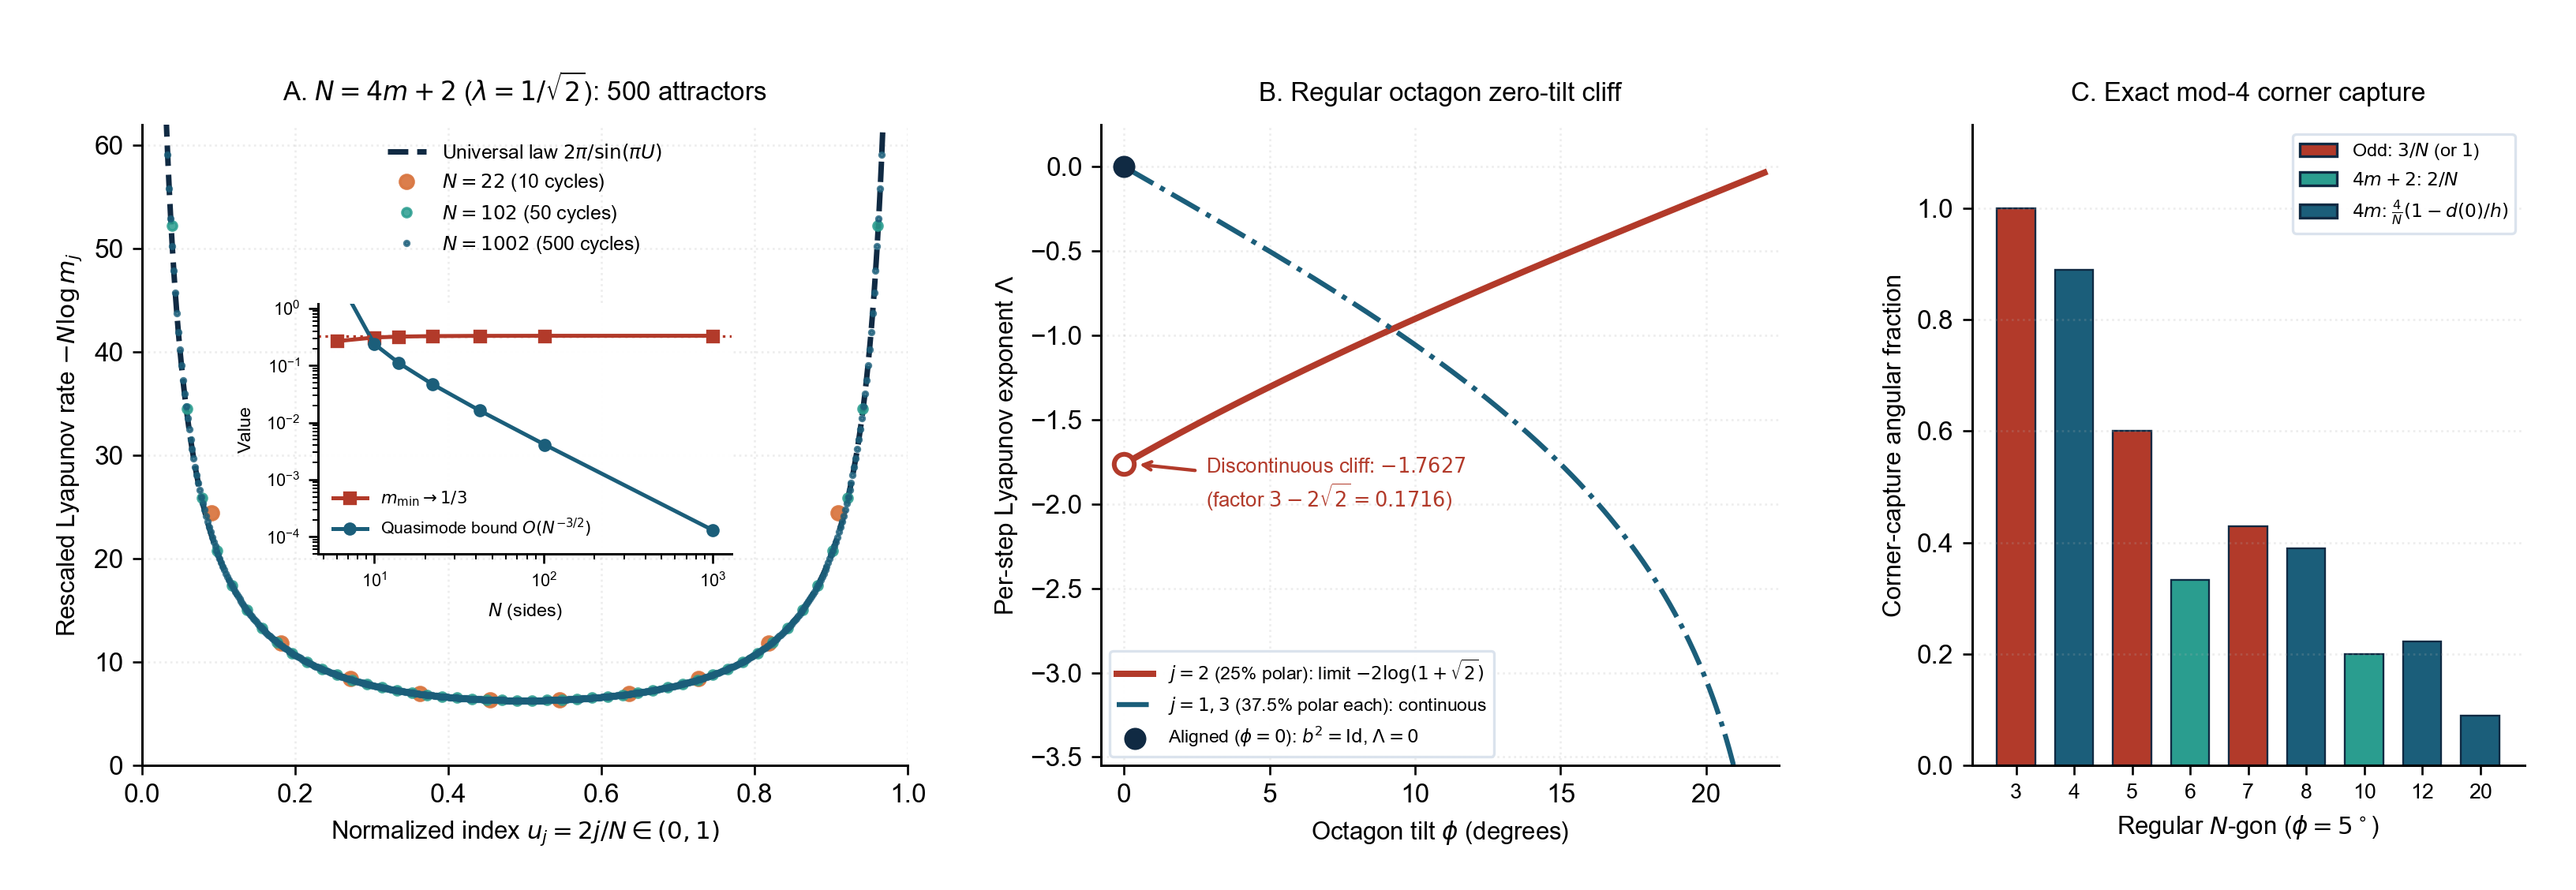
\includegraphics[width=\textwidth]{figs/p2_fig3_circle_paradox_and_octagon.png}
\caption{\textbf{A.} The Half-Frequency Paradox on aligned $N = 4m+2$ regular polygons ($\lambda = 1/\sqrt{2}$): on every interior quantile band $[\delta, 1-\delta]$ the rescaled rates $-N\log m_j$ approach $2\pi/\sin(\pi u)$ uniformly and $-N\ell_N \Rightarrow 2\pi/\sin(\pi U)$ under uniform boundary-arclength launch (the viewport clips the $32$ steepest endpoint cycles at $N=1002$, where $-N\log m_1 \approx 1100.8$ vs.\ $2\pi/\sin(2\pi/N) \approx 1002.0$, asymptotic ratio $\log 3$); inset shows the strongest factor staying pinned below $1/3$ ($m_{\min} \uparrow 1/3$) while the explicit $H_0^1$ ghost quasimode residual upper bound \eqref{eq:quasimode} drops as $O(N^{-3/2})$ ($\le 0.000130638$ at $N=1002$). \textbf{B.} Discontinuous zero-tilt Lyapunov cliff on the regular octagon: rotating by small $\phi \in (0, \pi/8)$ makes the $j=2$ basin ($25\%$ in polar angle) jump discontinuously onto $\log[\tan(\pi/8+\phi)/\tan(3\pi/8-\phi)]$, whose $\phi \downarrow 0$ limit is $-2\log(1+\sqrt{2}) = -1.762747\ldots$ \textbf{C.} Exact mod-$4$ corner-capture angular fractions \eqref{eq:mod4-corner} at $\phi = 5^\circ$.}
\label{fig:p2-fig3}
\end{figure}

% ==============================================================================
\section{Open Problems, Lean~4 Verification, and Reproducibility}\label{sec:open-lean}
% ==============================================================================

\subsection{Explicitly open boundaries}
Two sharp mathematical problems remain genuinely open beyond the theorems established here:
\begin{enumerate}
  \item \textbf{All-period regular-$N$-gon measure}: Theorem~\ref{thm:growing-Q} proves that all periods up to $Q_N = o(N/\sqrt{\log N})$ carry vanishing measure as $N \to \infty$, and reduces the complement of regular attractors (outside the corner bands) to the irrational-rotation set up to a countable set. Yet the \emph{total} Lebesgue measure of all-period regular attractors on a fixed regular $N$-gon ($N \ge 5$)---and its limit as $N \to \infty$---remains open (neither fixed-dilation two-break theorems \cite{LBC2023} nor Khmelev's dominant-break theorem \cite{Khmelev2005} apply when break locations and branch slopes co-vary).
  \item \textbf{Singular continuous spectral type on nonempty exceptional Cantor sets}: On a fixed tilted rectangle with $E_{R,\phi} \ne \varnothing$ (i.e., outside the extinction horn \eqref{eq:extinction}), Theorem~\ref{thm:measure-dim} characterizes $E_{R,\phi}$ as a Cantor set of dimension $1/2 < \dim_H E_{R,\phi} \le d_\phi < 1$ containing the countable dense set of eigenangles (those with odd boundary-rotation denominator). Setting $S_{R,\phi} = \{\cos^2\theta : \theta \in E_{R,\phi}\} \subset (0,1)$ for its spectral image, $S_{R,\phi}$ is Lebesgue-null, so every absolutely continuous spectral measure assigns it zero mass; determining whether the singular continuous spectral projection $\mathbf{1}_{S_{R,\phi}\setminus\sigma_p(T)}(T) P_{\mathrm{sc}}$ is nonzero remains open (cf.\ Fokin's smooth-domain singular-continuous constructions \cite{Fokin1994}).
\end{enumerate}

\subsection{Formal verification in Lean~4 and computational reproducibility}
Core algebraic, combinatorial, parity, extinction, microscopic-separation, bevel-multiplier, density-cancellation, and mod-$4$ arithmetic components of the theorems in this paper are formally verified in standalone \textbf{Lean~4.36.0} inside \texttt{studies/03-sobolev-wave-attractors/proofs/lean4/} (0 errors, 0 warnings, 0 \texttt{sorry}, standard axioms \texttt{propext}, \texttt{Classical.choice}, \texttt{Quot.sound} only; Table~\ref{tab:lean-p2}). Analytic regularity, physical realizability, measure-theoretic dimension bounds, and PDE quasimode estimates remain in the paper proofs.

\begin{table}[ht]
\centering
\caption{Machine-checked components of the cited theorems in standalone Lean~4.36.0 (\texttt{0 sorry}, standard axioms only).}
\label{tab:lean-p2}
\scriptsize
\setlength{\tabcolsep}{3.5pt}
\begin{tabular}{@{}>{\raggedright\arraybackslash}p{0.31\textwidth}l>{\raggedright\arraybackslash}p{0.43\textwidth}@{}}
\toprule
Result \& modeled component & Lean~4 module & Key verified declarations \\
\midrule
Thm.~\ref{thm:five-tanks} (4-tank model \& canonical return) & \texttt{TiltedParity} & \texttt{even\_boundary\_winding}, \texttt{odd\_boundary\_winding}, \texttt{canonical\_parity\_table}, \texttt{canonical\_physical\_identity\_iff}, \texttt{canonical\_regular\_interior\_iff} \\
Thm.~\ref{thm:extinction-reentry} \& Rem.~\ref{rem:zt} (extinction \& 12-piece witness) & \texttt{TiltedParity} & \texttt{extinction\_interval}, \texttt{extinction\_threshold}, \texttt{square\_extinction\_angle\_iff}, \texttt{square\_period\_two\_iff}, \texttt{zhang\_temnov\_cycles} \\
Thm.~\ref{thm:shaving} (separation, bevel \& rational density) & \texttt{CornerShavingAndTriangles} & \texttt{microscopic\_separation}, \texttt{at\_most\_one\_bevel\_visit}, \texttt{bevel\_return\_multiplier}, \texttt{period\_three\_midpoint\_multiplier}, \texttt{frequency\_density\_cancellation} \\
Thms.~\ref{thm:corner-shadow} \& \ref{thm:half-freq-paradox} (mod-4 \& rational bound) & \texttt{CornerShavingAndTriangles} & \texttt{regular\_corner\_fractions}, \texttt{minimumMultiplier\_lt\_third} \\
\bottomrule
\end{tabular}
\end{table}

All high-precision calculations (95-digit re-entry verification, exact integer tenth-power $9/10$ dimension certificate over $110{,}592$ triples, 122-case rational tongue verification, $39{,}797$ shaving plateaus at $\varepsilon = 1/512$, and regular-$N$-gon interval audits) are reproduced deterministically by the scripts in \texttt{experiments/}: \texttt{phase1\_\allowbreak canonical.py}, \texttt{phase1\_\allowbreak measure.py}, \texttt{phase1\_\allowbreak rectangle.py}, \texttt{phase1\_\allowbreak pde.py}, \texttt{phase1\_\allowbreak regular.py}, \texttt{test\_\allowbreak phase1\_\allowbreak repairs.py}, and \texttt{generate\_\allowbreak paper\_\allowbreak figures.py}.

\begin{thebibliography}{99}

\bibitem{Aleksandryan1960}
R.~A.~Aleksandryan,
\emph{Spectral properties of operators generated by systems of differential equations of S.~L.~Sobolev type} (Russian),
Trudy Moskov.\ Mat.\ Obshch.\ \textbf{9} (1960), 455--505 (building on 1949 Moscow State Univ.\ dissertation).

\bibitem{BajarsFrankMaas2013}
J.~Bajars, J.~Frank, and L.~R.~M.~Maas,
\emph{On the appearance of internal wave attractors due to an initial or parametrically excited disturbance},
J.\ Fluid Mech.\ \textbf{714} (2013), 283--311.

\bibitem{BoulangerGhazouaniTahar2025}
A.~Boulanger, S.~Ghazouani, and G.~Tahar,
\emph{Closed geodesics in dilation surfaces},
Geom.\ Topol.\ \textbf{29} (2025), no.~4, 2217--2250.

\bibitem{CdVSR2020}
Y.~Colin de Verdi\`ere and L.~Saint-Raymond,
\emph{Attractors for two-dimensional waves with homogeneous Hamiltonians of degree~$0$},
Comm.\ Pure Appl.\ Math.\ \textbf{73} (2020), no.~2, 421--462.

\bibitem{DyatlovZworski2019}
S.~Dyatlov and M.~Zworski,
\emph{Microlocal analysis of forced waves},
Pure Appl.\ Anal.\ \textbf{1} (2019), no.~3, 359--384.

\bibitem{DWZ2025}
S.~Dyatlov, J.~Wang, and M.~Zworski,
\emph{Mathematics of internal waves in a two-dimensional aquarium},
Anal.\ PDE \textbf{18} (2025), no.~1, 1--92.

\bibitem{Fokin1994}
M.~V.~Fokin,
\emph{Existence of the singular spectrum and asymptotic behavior of solutions in Sobolev's problem} (Russian),
Trudy Inst.\ Mat.\ SO RAN \textbf{26} (1994), 107--195.

\bibitem{Khmelev2005}
D.~Khmelev,
\emph{Rational rotation numbers for homeomorphisms with several break-type singularities},
Ergodic Theory Dynam.\ Systems \textbf{25} (2005), 553--592.

\bibitem{Kopecz2006}
S.~Kopecz,
\emph{Fractal internal wave patterns in a tilted square},
Student training report, CWI (Centrum Wiskunde \& Informatica) in cooperation with NIOZ, 2006.

\bibitem{LBC2023}
M.~Lenci, C.~Bonanno, and G.~Cristadoro,
\emph{Internal-wave billiards in trapezoids and similar tables},
Nonlinearity \textbf{36} (2023), 1029--1052.

\bibitem{Li2024}
Z.~Li,
\emph{Internal waves in aquariums with characteristic corners},
arXiv:2402.01896 (2024).

\bibitem{MaasLam1995}
L.~R.~M.~Maas and F.-P.~A.~Lam,
\emph{Geometric focusing of internal waves},
J.\ Fluid Mech.\ \textbf{300} (1995), 1--41.

\bibitem{Maas1997}
L.~R.~M.~Maas, D.~Benielli, J.~Sommeria, and F.-P.~A.~Lam,
\emph{Observation of an internal wave attractor in a confined, stably stratified fluid},
Nature \textbf{388} (1997), 557--561.

\bibitem{NogueiraTroubetzkoy2020}
A.~Nogueira and S.~Troubetzkoy,
\emph{Chess billiards},
arXiv:2007.14773 (2020).

\bibitem{Paper1}
Project ReMath,
\emph{Uncloakable Standing Waves and Prescribed Multi-Attractor Coexistence in Polygonal Sobolev Tanks},
Study~\#03 Companion Preprint (Paper~1), November 2026.

\bibitem{Soares2021}
L.~Soares,
\emph{Hecke triangle groups, transfer operators and Hausdorff dimension},
Ann.\ Henri Poincar\'e \textbf{23} (2022), 1239--1281 (published online 2021).

\bibitem{Sobolev1954}
S.~L.~Sobolev,
\emph{On a new problem of mathematical physics} (Russian),
Izv.\ Akad.\ Nauk SSSR Ser.\ Mat.\ \textbf{18} (1954), no.~1, 3--50.

\bibitem{Zelenyak1965}
T.~I.~Zelenyak,
\emph{On the boundary dependence of solutions of some mixed problems for the equations of small oscillations of a rotating fluid} (Russian),
Dokl.\ Akad.\ Nauk SSSR \textbf{164} (1965), no.~6, 1225--1228.

\bibitem{Zelenyak1970}
T.~I.~Zelenyak,
\emph{Selected Questions of the Qualitative Theory of Partial Differential Equations} (Russian),
Novosibirsk State University, Novosibirsk, 1970.

\bibitem{ZhangTemnov2026}
Y.~Zhang and A.~N.~Temnov,
\emph{Spectral properties of the internal wave operator in nonclassical problems},
Contemp.\ Math.\ Fundam.\ Dir.\ \textbf{72} (2026), no.~2, 368--387.

\bibitem{ZhuLi2022}
S.~Zhu (under the direction of Z.~Li),
\emph{On the smoothness and regularity of the chess billiard flow and the Poincar\'e problem},
arXiv:2210.13384 (2022).

\end{thebibliography}

\end{document}
